\documentclass[12pt
,a4paper
,titlepage
,twoside
%,openany % ouvre les sections indifféremment sur la page de gauche ou de droite
]{book}

% Définition des marges de la page
\usepackage[left=3cm,right=3cm,top=2cm,bottom=2cm]{geometry}

% Paramétrages de la langue et de l'encodage
\usepackage[utf8x]{inputenc}
\usepackage[square,sort,comma,numbers]{natbib}
\usepackage[french]{babel}
\usepackage[T1]{fontenc}

%\usepackage{fontspec}
%\setmainfont{Linotype-AvenirNextLTPro.ttf}[
%BoldFont = Linotype-AvenirNextLTProBold.ttf,
%ItalicFont = Linotype-AvenirNextLTProItalic.ttf,
%BoldItalicFont = fLinotype-AvenirNextLTProBoldItalic.ttf
%]

% formules mathématiques
\usepackage{amsmath}
\usepackage{amsfonts}
\usepackage{amssymb}

% gestion des graphiques
\usepackage{graphicx}
\usepackage{transparent}

% Gestion des couleurs
\usepackage[usenames,dvipsnames]{xcolor}
\definecolor{inrae}{RGB}{0,163,166} % inrae
\definecolor{inraeclair}{RGB}{102,193,191}   % inrae clair
\definecolor{inraemedium}{RGB}{0,140,142}   % inrae medium
\definecolor{inraefonce}{RGB}{39,86, 98} % inrae foncé
\definecolor{vert}{RGB}{157,197,68} % vert
\definecolor{bleuclair}{RGB}{158,214,227} % bleu clair
\definecolor{bleufonce}{RGB}{66,48,137} % bleu foncé
\definecolor{gris}{RGB}{121,120,112}   % gris
\definecolor{argent}{RGB}{196,192,179} % argent
\definecolor{rouge}{RGB}{142,2,0} % rouge

% Redefinition des liens web
\usepackage{url}
\usepackage{hyperref}
\hypersetup{
urlcolor=inraefonce
,linkcolor=.
,colorlinks=true}


% Polices de caractères
\usepackage{times}
\usepackage{mathptmx} % times, y compris dans les formules mathématiques
\renewcommand{\familydefault}{\sfdefault}

% Insertion de code source dans le texte, à utiliser avec \begin{lstlisting} et \lstset{java|html|php...}
\usepackage{listings}
\lstset{
basicstyle=\footnotesize,        % the size of the fonts that are used for the code
  breakatwhitespace=false,         % sets if automatic breaks should only happen at whitespace
  breaklines=true,
  keepspaces=true,
}

% Définition des entêtes
\usepackage{fancyhdr}
\pagestyle{fancy}

% Redéfinition des titres de section
\usepackage{titlesec}

% Insertion de graphiques à des emplacements définis
\usepackage[abs]{overpic}

% règles typographiques de l'Imprimerie nationale
\usepackage[all]{nowidow}
\usepackage[
% frenchchapters renomme le premier chapitre, mais :
%	- cela pose problème dans la table des matières
%	- cela ne peut être utilisé qu'avec la renumérotation des chapitres activée
%frenchchapters,
parindent,
lastparline,
hyphenation
]{impnattypo}

% Renumérotation des chapitres
%\renewcommand{\thesection}{\Alph{section})}
%\renewcommand{\thesubsection}{\arabic{subsection} -}
%\renewcommand{\thesubsubsection}{\alph{subsubsection} -}
%\usepackage{engrec}
%\renewcommand{\theparagraph}{\engrec{paragraph})}
%\setcounter{secnumdepth}{4}

% Génération du code Ipsum lorem
\usepackage{blindtext}


% Definition des chapitres
%\usepackage{sectsty}
\titleformat{\chapter}[display]
{\normalfont\Huge\filcenter\sffamily\color{inrae}}
{\Large{\chaptertitlename~\thechapter}}
 {1em}{}

%{\titlerule
%% \vspace{1pc}%


\titleformat{\section}
{\color{inrae}\normalfont\Large\bfseries\sffamily}
{\color{inrae}\thesection}{1em}{}

\titleformat{\subsection}
{\color{inraefonce}\bfseries\sffamily}
{\color{inraefonce}\thesubsection}{1em}{}

\titleformat{\subsubsection}
{\color{gris}\bfseries\sffamily}
{\color{gris}\thesubsubsection}{1em}{}

% Bibliographie
% natbib est indispensable si la biblio contient des accents
% Options pour natbib (extrait de http://merkel.zoneo.net/Latex/natbib.php)
%    round: (par défaut) pour des parenthèses arondies (());
%    square: pour des crochets ([]);
%    curly: pour des accolades ({});
%    angle: pour des équerres (<>) ;
%    colon: (par défaut) pour séparer les citations multiples par deux points (:);
%    comma: pour utiliser une virgule comme séparateur;
%    authoryear: (par défaut) pour des citations auteurs-année;
%    numbers: pour des citations numériques;
%    super: pour des citations numériques en exposant, comme dans Nature;
%    sort: ordonne les citations multiples dans l'ordre dans lequel elles apparaissent dans la bibliographie;
%    sort&compress: comme sort mais en plus les citations numériques multiples sont comprimées, si possible (3-6, 15, par exemple);
%    longnamesfirst: transforme la première citation à une référence en une version étoilée (avec la liste complète des auteurs) et le citations suivantes normales (liste abbrégée);
%    sectionbib: pour redéfinir \thebibliography pour avoir une \section* à la place d'un \chapter*; valide seulement pour les classes de document possédant la commande \chapter; à utiliser avec le paquetage  chapterbib;
%    nonamebreak: garde tous les noms d'auteurs d'une citation sur une même ligne; celà cause des problèmes de débordement, mais permet de résoudre certains problèmes liés à hyperref.

% En cas de souci, supprimez les fichiers .aux et .bbi après modification des paramètres
% styles natbib natifs : abbrvnat, plainnat, unsrtnat
\bibliographystyle{unsrtnat}
\usepackage{hypernat}
% Ajout de la référence à la bibliographie dans la table des matières
\usepackage[nottoc, notlof, notlot]{tocbibind}

%Données de titre et d'auteur pour la page de garde
\newcommand{\titre}{Logiciel Collec-Science}
\newcommand{\sousTitre}{Installation, configuration et administration}
\newcommand{\auteur}{Éric Quinton}
\newcommand{\dateVersion}{1\ier{} mars 2020}
\newcommand{\version}{Version 2.4.0}
\usepackage[final]{pdfpages} 

\usepackage{lscape}
\usepackage{longtable}
\usepackage{float}
\usepackage{array}
\begin{document}
%Supprime les veuves et orphelines
\widowpenalty=10000
\clubpenalty=10000
\raggedbottom 

% Integrer la page de garde
\input{page_de_garde}
% Définition des entêtes
\fancyhead{}
\fancyhead[CO]{\leftmark\sffamily}
\fancyhead[CE]{ \sffamily\titre{}}
\fancyfoot[CO]{\sffamily\thepage}
\fancyfoot[CE]{\sffamily\thepage}
% Redéfinition de \cleardoublepage pour créer une page totalement vide
\makeatletter
\def\cleardoublepage{\clearpage\if@twoside \ifodd\c@page\else
  \hbox{}
  \vspace*{\fill}

  \vspace{\fill}
  \thispagestyle{empty}
  \newpage
  \if@twocolumn\hbox{}\newpage\fi\fi\fi}
\makeatother

% \cleardoublepage permet de générer une page vide 
% si le chapitre ne commence pas sur la page de droite

% Ajout d'un préambule
\frontmatter
\cleardoublepage

% Table des matières
\tableofcontents


% Début réel du texte
\mainmatter
%\cleardoublepage

\chapter{Besoins nécessitant l'utilisation de services web}

\section{Définitions}

\begin{description}
\item[uid:] identifiant unique numérique au sein d'une base de données d'un échan\-tillon ;
\item[guid:] identifiant de type UUID\footnote{Les codes de type GUID ou UUID sont générés à partir de fonctions aléatoires ou cryptographiques, et garantissent qu'ils sont uniques quelle que soit la base de données qui les ont générés. Ainsi, il n'est pas possible d'obtenir deux codes identiques pour deux échantillons différents, ce qui permet de les identifier de manière sûre, comme pourrait le faire l'ADN pour des êtres humains.}, qui garantit de manière certaine l'identification d'un échantillon ;
\item [identifier :] identifiant \og métier \fg{} d'un échantillon;
\item [données \og métier \fg{} :] données permettant de caractériser un échantillon selon les critères nécessaires à son exploitation : contexte spécifique d'acquisition, taxon, données physico-chimiques ou biologiques, etc.
\item [instance, serveur, base de données, application :] implémentation d'une solution de gestion d'échantillons capable soit de fournir des services web, soit d'interroger des services web pour récupérer des informations.
\end{description}
\section{Présentation}

La gestion des échantillons de laboratoire (ou autres) est réalisée par divers logiciels, chacun s'appuyant sur une base de données différente. Dans un contexte d'échange des informations entre laboratoires, il est apparu nécessaire de proposer une méthode d'interrogation des différentes bases de données, pour connaître ce qui est disponible dans d'autres collections.

Deux cas d'utilisation ont ainsi pu être mis en évidence :
\begin{itemize}
\item l'interrogation d'une base distante, pour savoir si des échantillons sont disponibles ;
\item l'import d'informations provenant d'une autre base de données, pour ré\-pondre à deux cas de figure différents :
\begin{itemize}
\item le prêt d'un échantillon à un autre laboratoire, sans être obligé de ressaisir toutes les métadonnées associées ;
\item l'importation de données saisies sur le terrain en mode déconnecté dans une base de données centrale.
\end{itemize}
\end{itemize}

La technologie retenue est celle des services web, associée au protocole OAuth v.2 pour la gestion des habilitations.

\subsection{Technique employée}

Les services web sont basés sur des requêtes HTTP, et échangent les données selon des formats définis. Dans la version actuelle des services web, seul le format Json est implémenté pour l'échange des informations.

\subsection{Forme des URL}
Les URL sont conçues, dans le cadre des services web, sous la forme d'URL conviviales, par exemple : \textit{http://collec/sw/v1/sample/4} pour récupérer l'échan\-tillon numéro 4.

\section{Définition des cas d'utilisation couverts par les services web}

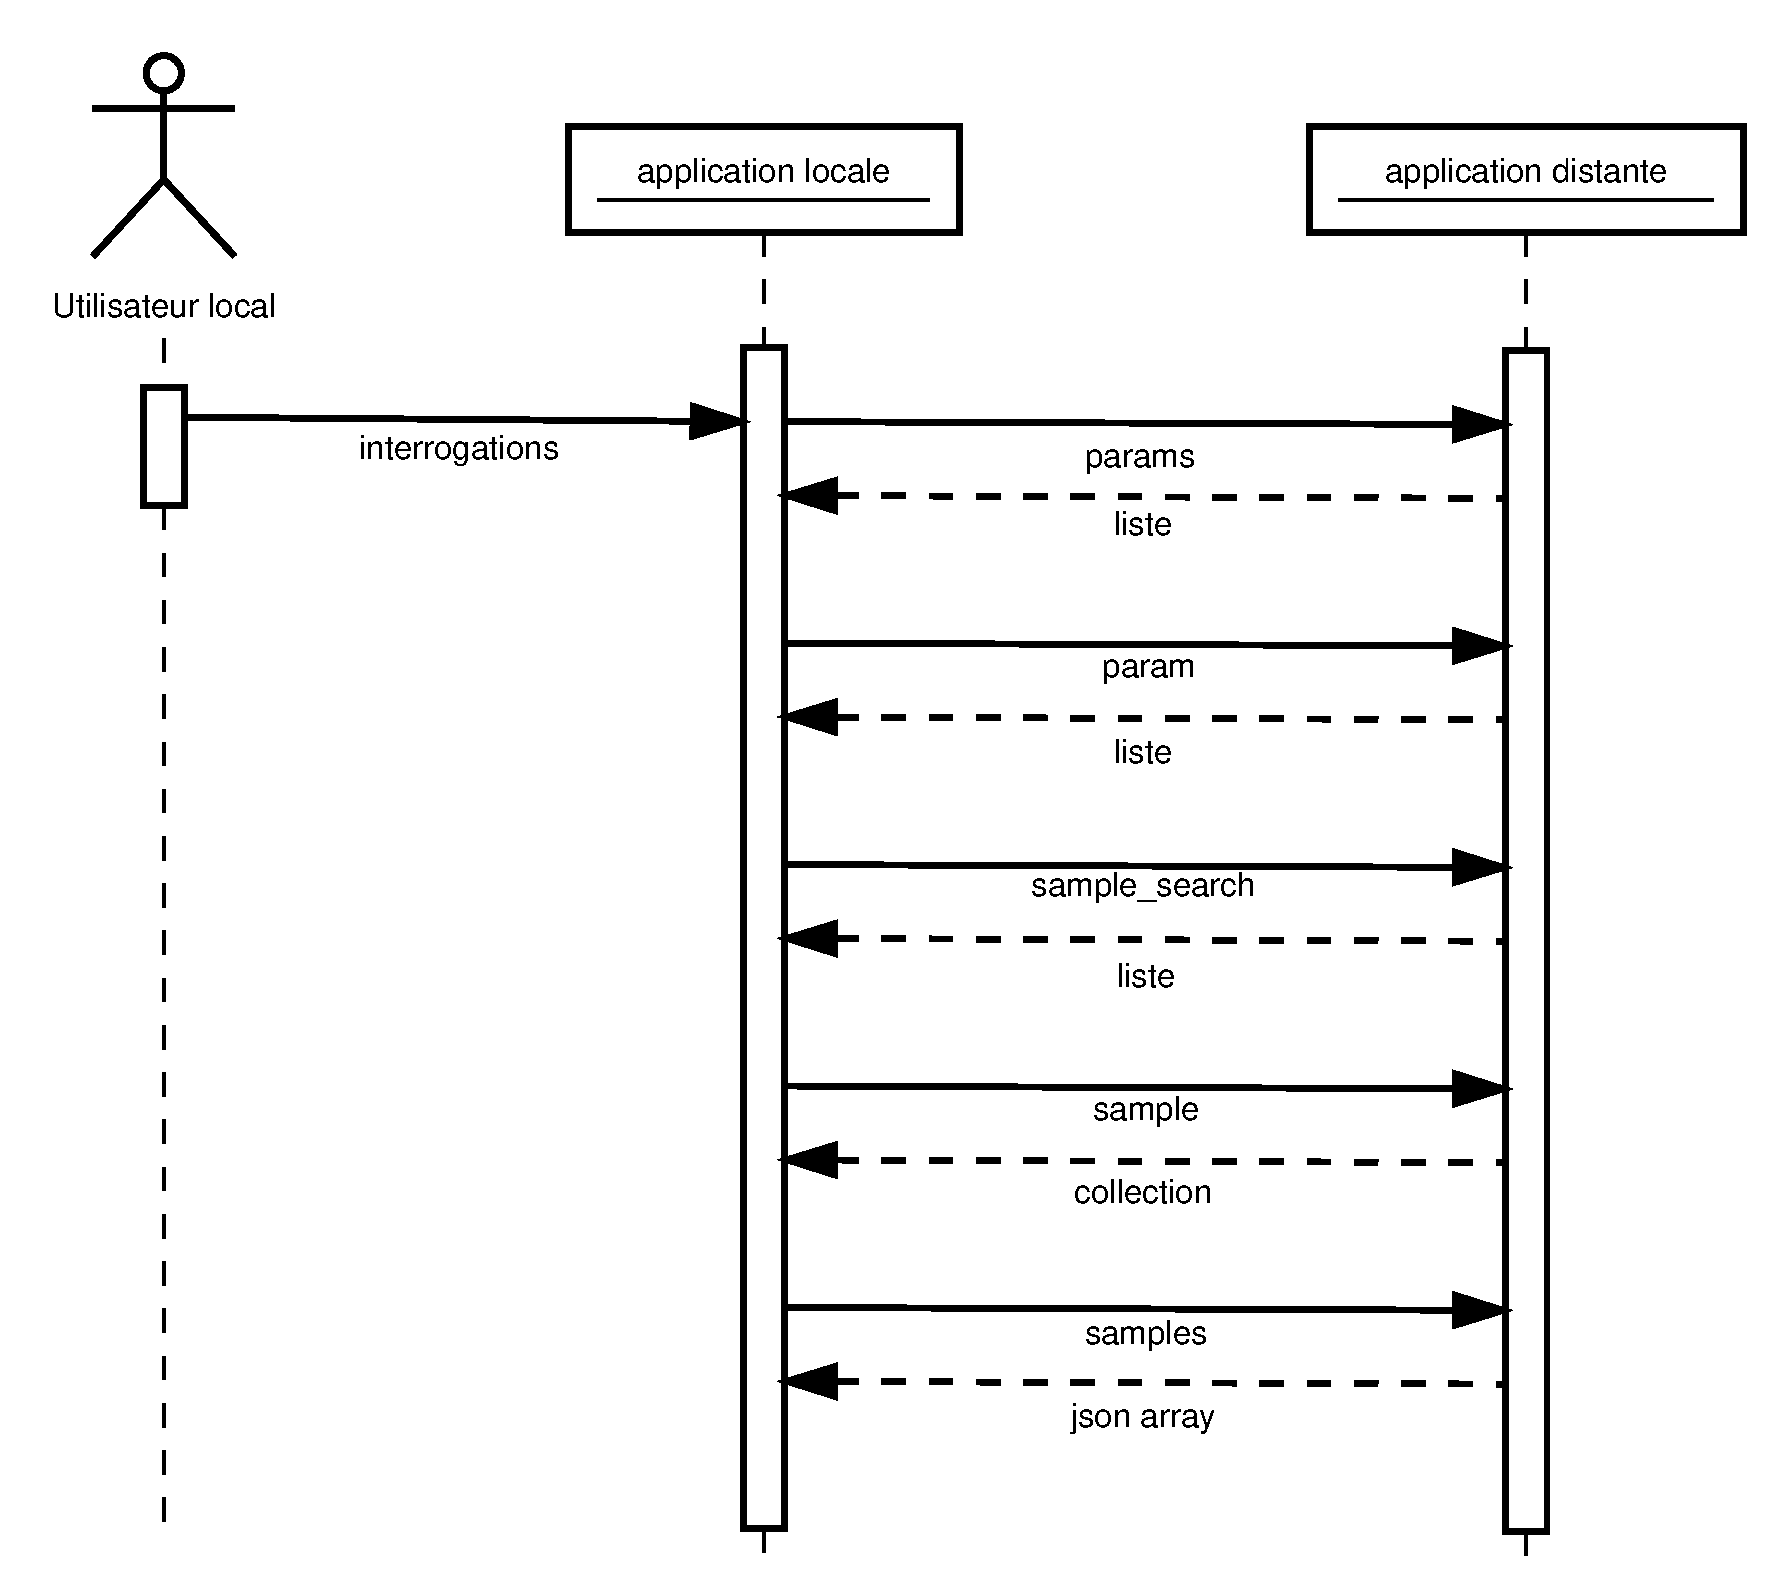
\includegraphics[width=\linewidth]{images/sequence}

Cinq services web sont nécessaires :
\begin{itemize}
\item les deux premiers permettent de récupérer les listes de référence nécessaires pour faire des recherches selon divers paramètres ;
\item le troisième permet de lancer une recherche pour trouver des échantillons ;
\item les deux derniers récupèrent les informations correspondant à un ou plusieurs échantillons respectivement.
\end{itemize}


\subsection{Recherche d'échantillons}
La recherche d'échantillons doit pouvoir s'effectuer selon plusieurs critères :
\begin{itemize}
\item l'identifiant interne (\textit{uid});
\item l'identifiant principal ou des identifiants secondaires;
\item une fourchette de dates de création des échantillons;
\item un type d'échantillons;
\item un projet ou sous-collection;
\item une fourchette d'identifiants internes;
\item un code unique de type GUID ou UUID;
\item le lieu de collecte de l'échantillon;
\item tout autre paramètre traité dans l'application distante.
\end{itemize}

Elle retourne une liste d'échantillons correspondant aux critères indiqués. Le détail des informations retournées est spécifié dans la section \ref{sampleSearch}.

Pour permettre cette recherche, il est nécessaire de récupérer les tables de référence (types d'échantillons, projets ou sous-collections, lieux de collecte...). Les tables utilisables pour la recherche peuvent différer selon les logiciels, et cette liste peut être retrouvée par un service web dédié.

\subsection{Liste des tables de référence}
Ce service permet d'obtenir l'ensemble des tables de référence avec lesquelles il est possible de réaliser une recherche.

\subsection{Contenu des tables de référence}
Ce service récupère le contenu d'une des tables de référence.

\subsection{Récupération des données d'un échantillon}
Ce service permet de récupérer l'ensemble des données concernant un échan\-tillon, y compris les données \og métiers \fg{} si l'utilisateur dispose des droits néces\-saires pour les consulter.

Les données récupérées doivent être suffisamment complètes pour être intégrées dans l'application de gestion des échantillons locale.

Elles permettent également une visualisation détaillée de l'échantillon consi\-déré, et contiennent, le cas échéant\footnote{si l'utilisateur dispose des droits adéquats et si l'échantillon dispose de ces informations}, les données \og métiers \fg{} associées.

\subsection{Récupération des données d'une liste d'échantillons}

Il s'agit d'une variante du service web précédent. La liste des échantillons à récupérer est fournie dans une collection Json, soit en utilisant l'UID, soit en utilisant le GUID.

\section{Contraintes liées à la sécurité}

L'accès aux données nécessite une identification préalable de l'utilisateur. Celle-ci est basée sur le protocole OAuth v2 (\textit{cf.} chapitre \ref{oauth}).



\chapter{Installer le logiciel}

\section{Consultez la documentation du framework !}

Le logiciel a été conçu à partir du framework \textit{Prototypephp}. La documentation associée \cite{pphp-doc} récapitule l'ensemble des informations nécessaires pour réaliser l'installation générale (configuration du serveur, définition des droits d'accès, etc.).

De nombreuses reprises figurent ici, mais il n'est pas inutile de se référer au document d'origine. Seuls les exemples dédiés au logiciel sont présentés, mais d'autres informations utiles pourront y être piochées.

\section{Configuration du serveur}
La configuration est donnée pour un serveur Linux fonctionnant avec Ubuntu 16.04 LTS Server. Elle peut bien sûr être adaptée à d'autres distributions Linux. Par contre, rien n'a été prévu pour faire fonctionner l'application directement dans une plate-forme windows, même si, en théorie, cela devrait être possible.

\subsection{Configuration d'Apache}
Les modules suivants doivent être activés :
\begin{lstlisting}
a2enmod ssl
a2enmod headers
a2enmod rewrite
\end{lstlisting}

\subsection{Modules PHP nécessaires}
Modules complémentaires nécessaires :
\begin{itemize}
\item \textit{php-mbstring}
\item \textit{php-pgsql}
\item \textit{php-xdebug} pour les phases de mise au point.
\end{itemize}
La génération des étiquettes nécessite les paquetages suivants :
\begin{itemize}
\item \textit{php-gd} (ou \textit{php5-gd} pour les serveurs en version 5)
\item \textit{fop} (qui inclut des bibliothèques java)
\end{itemize}

Le stockage et l'affichage des photos nécessite :
\begin{itemize}
\item \textit{php-imagick} (ou \textit{php5-imagick} pour les serveurs en version 5)
\end{itemize}

\subsection{Configuration de l'hôte virtuel et de SSL}
L'application ne fonctionne qu'en mode SSL, les cookies de session n'étant pas transmis sur des liens non chiffrés. Voici un exemple de configuration à insérer dans le fichier \textit{/etc/apache2/sites-available/default-ssl}
\begin{lstlisting}
    <Directory /var/www/html>
        Options FollowSymLinks MultiViews
        AllowOverride all
        Order allow,deny
        allow from all
    </Directory>

    SSLProtocol All -SSLv2 -SSLv3
    SSLHonorCipherOrder On
    SSLCipherSuite ECDHE-RSA-AES128-SHA256:AES128-GCM-SHA256:HIGH:!MD5:!aNULL:!EDH:!RC4
    SSLCompression off
\end{lstlisting}

La chaîne \textit{SSLCipherSuite} est donnée à titre d'exemple, d'autres configurations plus modernes peuvent être implémentées \cite{tls}.

Pour activer le mode SSL dans Apache :
\begin{lstlisting}
chmod -R g+r /etc/ssl/private
usermod www-data -a -G ssl-cert
a2ensite default-ssl
service apache2 restart
\end{lstlisting}


\subsection{Configuration du dossier d'installation}

\subsubsection{Mécanisme pour faire cohabiter plusieurs instances avec le même code}

Il est possible d'utiliser le même code applicatif pour alimenter des bases de données différentes (ou des données stockées dans des schémas différents). Cette fonctionnalité est basée sur l'attribution d'entrées DNS différentes. 

Le mécanisme est décrit dans le schéma \ref{dnsmultiple}, page \pageref{dnsmultiple}.

\begin{figure}[H]
\label{dnsmultiple}
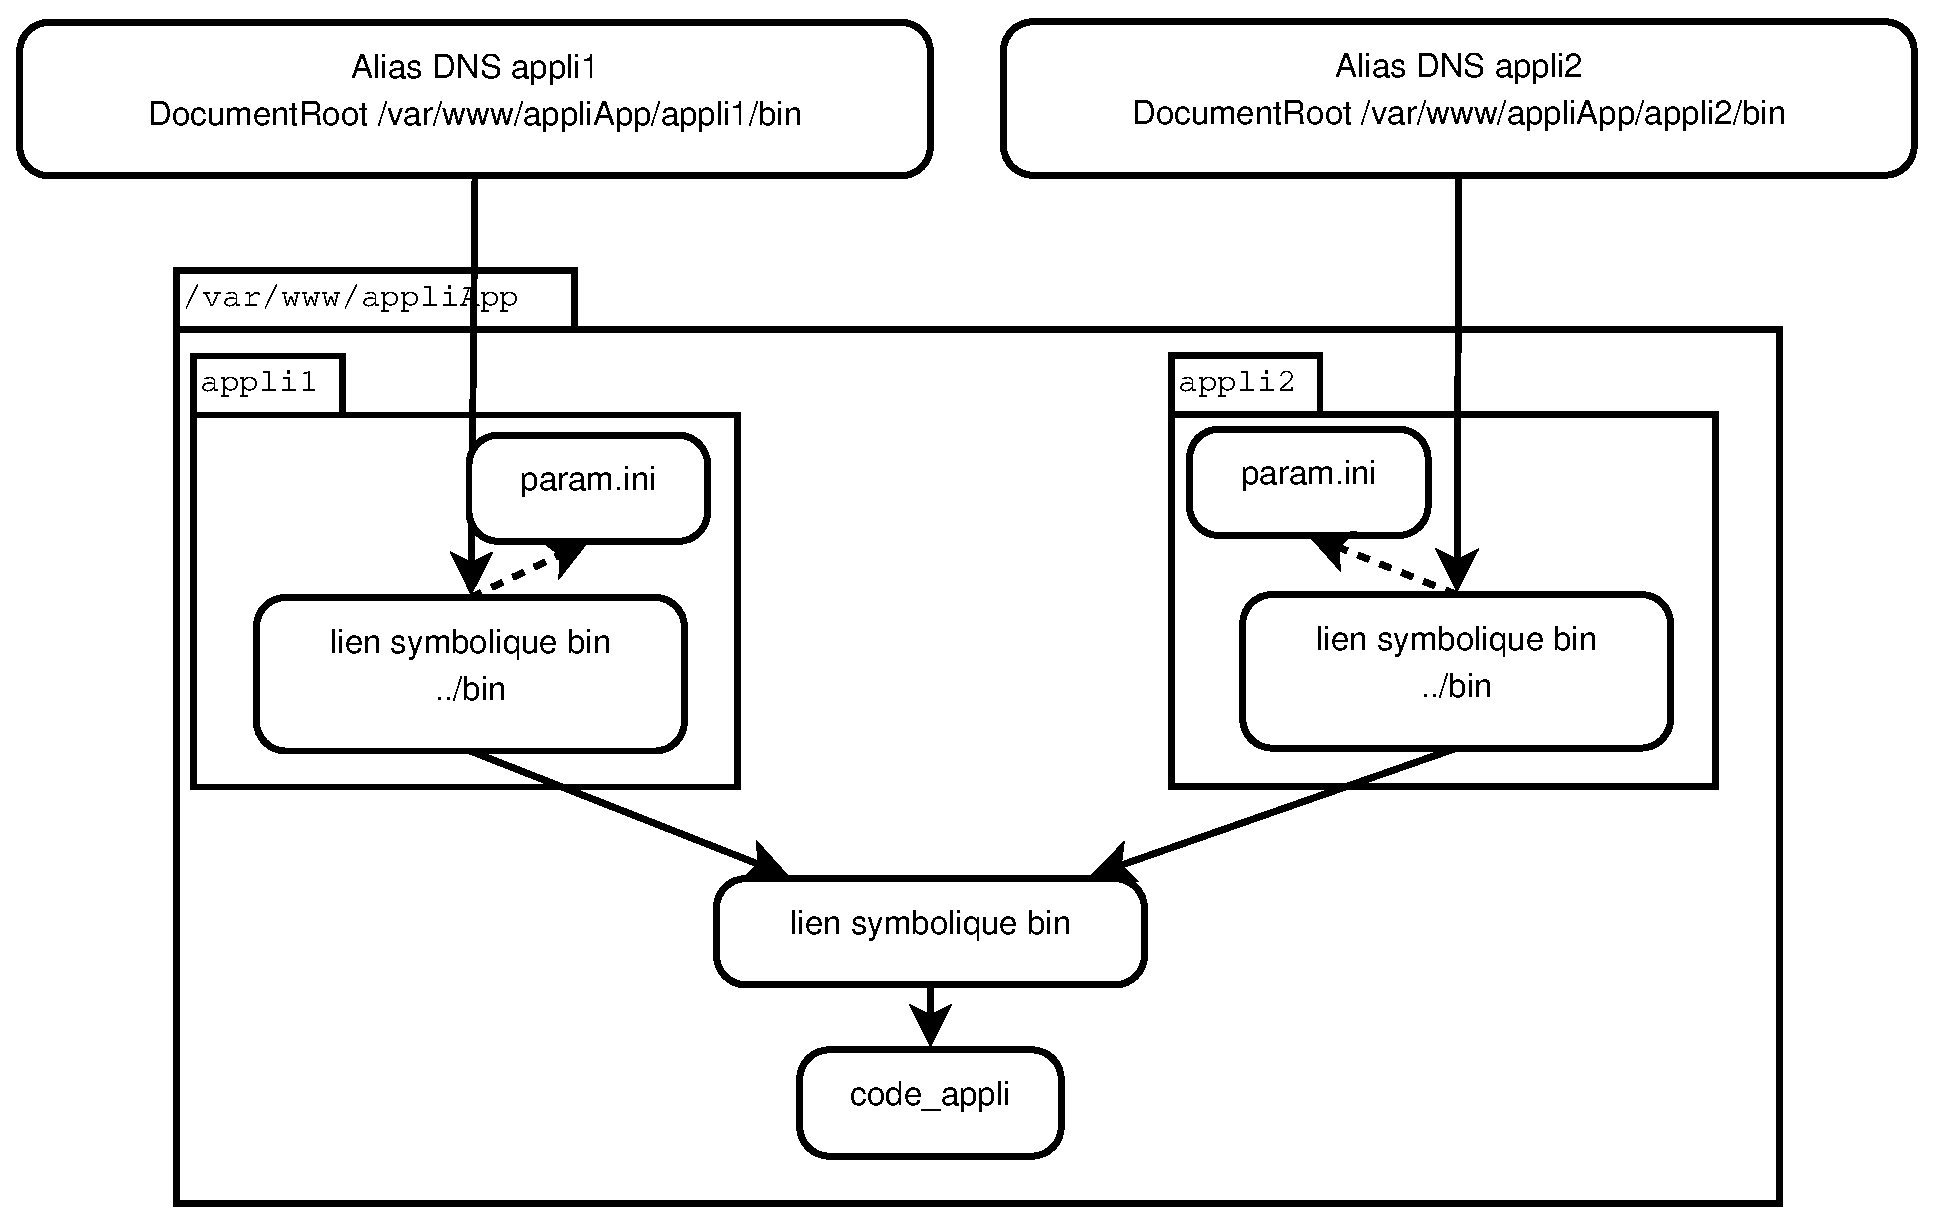
\includegraphics[width=\linewidth]{images/dnsmultiple}
\caption{Schéma général d’implémentation pour utiliser le même code avec des noms d’application et des jeux de données différents}
\end{figure}

Dans le paramétrage de l’alias DNS (en principe, dans \textit{/etc/apache2/sites-available}), l’application pointe vers le dossier \textit{/var/www/appliApp/appli1/bin}. \textit{/var/www} correspond à la racine du site web, \textit{appliApp} au dossier racine de l’application, \textit{appli1} au dossier spécifique de l’alias DNS. Ce dossier \textit{appli1} ne contient que deux fichiers : \textit{param.ini}, qui contient les paramètres spécifiques, et \textit{bin}, qui est un lien symbolique vers le dossier \textit{../bin}.

Le dossier \textit{../bin} (donc, dans\textit{ /var/www/appliApp}) est lui aussi un alias qui pointe vers le code réel de l’application, ici \textit{code\_appli}. Le fichier \textit{param.inc.php} décrit l’entrée suivante : 
\begin{lstlisting}
$paramIniFile = "../ param . ini "; 
\end{lstlisting}

Le fichier \textit{param.ini} sera cherché dans le dossier parent du code de l’application, c’est à dire soit dans \textit{appli1}, soit dans \textit{appli2} dans cet exemple. Il suffit qu’il contienne les paramètres adéquats pour rendre l’application utilisable dans des contextes différents à partir du même code initial.



Le fichier \textit{param.ini} est le dernier qui est traité par l'application pour récupérer les paramètres.Ceux-ci sont lus dans l'ordre suivant :

\textbf{param/param.default.inc.php $\rightarrow$ param/param.inc.php $\rightarrow$ ../param.ini}

\textit{param.ini} contiendra les entrées spécifiques liées au DNS utilisé pour accéder à l'application, en principe tout ou partie de celles-ci :
\begin{lstlisting}
APPLI_titre=Gestion des collections EABX
BDD_schema=col, public, gacl
BDD_login=compte_de_connexion
BDD_passwd=mot_de_passe_de_connexion
BDD_dsn=pgsql:host=serveur;dbname=base_de_donnees;sslmode=require
GACL_aco=col
APPLI_code=proto
\end{lstlisting}



\subsubsection{Droits à attribuer au serveur web}

\section{Configurer l'application}

L'application est configurable par l'intermédiaire de trois fichiers, comme nous venons de le voir :

\textbf{param/param.default.inc.php $\rightarrow$ param/param.inc.php $\rightarrow$ ../param.ini}

Le premier fichier contient les paramètres par défaut. Il est systématiquement fourni à chaque nouvelle version de l'application.

Le second est spécifique de l'implémentation. Il comprend notamment les informations liées à la connexion à la base de données, à la méthode d'identification, ou à la recherche des attributs dans l'annuaire LDAP. 

le troisième est destiné à traiter la possibilité d'accéder, à partir du même code applicatif, à plusieurs bases de données différentes (\textit{cf.} \ref{dnsmultiple} \textit{\nameref{dnsmultiple}}).

Voici les principaux paramètres utilisés :

\subsection{Connexion à la base de données}

Dans la pratique, deux connexions sont nécessaires : l'une pour accéder à la base des droits, l'autre aux données proprement dites. Voici les paramètres à définir :

\begin{longtable}{|p{5cm}|p{10cm}|}
\hline
\textbf{Variable} & \textbf{Signification} \\
\hline
\endhead
BDD\_login & compte de connexion à la base de données \\
\hline
BDD\_passwd & mot de passe associé\\
\hline
BDD\_dsn & adresse de la base de données sous forme normalisée\\
\hline
BDD\_schema & schéma utilisé (plusieurs schémas peuvent être décrits, en les séparant par une virgule - fonctionnement propre à Postgresql)\\
\hline
GACL\_dblogin & compte de connexion à la base de données des droits\\
\hline
GACL\_dbpasswd & mot de passe associé\\
\hline
GACL\_dsn & adresse normalisée \\
\hline
GACL\_schema & schéma utilisé\\
\hline
GACL\_aco & nom du code de l'application utilisé dans la gestion des droits\\
\hline
\caption{Variables utilisées pour paramétrer les connexions}
\end{longtable}

\subsection{Identification des utilisateurs}

\begin{longtable}{|p{5cm}|p{10cm}|}
\hline
\textbf{Variable} & \textbf{Signification} \\
\hline
\endhead
ident\_type & Type d'identification supporté. L'application peut gérer \textbf{BDD} (uniquement en base de données),\textbf{LDAP} (uniquement à partir d'un annuaire LDAP) \textbf{LDAP-BDD} (d'abord identification en annuaire LDAP, puis en base de données), et \textbf{CAS} (serveur d'identification \textit{Common Access Service})\\
\hline
CAS\_plugin & Nom du plugin utilisé pour une connexion CAS \\
\hline
CAS\_address & Adresse du serveur CAS\\
\hline
CAS\_port & Systématiquement 443 (connexion chiffrée)\\
\hline
LDAP & tableau contenant tous les paramètres nécessaires pour une identification LDAP \\
\hline
privateKey & clé privée utilisée pour générer les jetons d'identification \\
\hline
pubKey & clé publique utilisée pour générer les jetons d'identification \\
\hline
tokenIdentityValidity & durée de validité, en secondes, des jetons d'identification\\
\hline
\caption{Variables utilisées pour paramétrer l'identification}
\end{longtable}

\subsection{Configuration de l'accès à l'annuaire LDAP}

Les paramètres LDAP sont stockés dans un tableau :
\begin{lstlisting}
$LDAP = array(
		"address"=>"localhost",
		"port" => 389,
		"rdn" => "cn=manager,dc=example,dc=com",
		"basedn" => "ou=people,ou=example,o=societe,c=fr",
		"user_attrib" => "uid",
		"v3" => true,
		"tls" => false,
		"groupSupport"=>true,
		"groupAttrib"=>"supannentiteaffectation",
		"commonNameAttrib"=>"displayname",
		"mailAttrib"=>"mail",
		'attributgroupname' => "cn",
		'attributloginname' => "memberuid",
		'basedngroup' => 'ou=example,o=societe,c=fr'
);
\end{lstlisting}


L'application peut non seulement identifier les utilisateurs auprès de l'annuaire LDAP, mais également récupérer les groupes auxquels ils appartiennent dans celui-ci.

Voici les paramètres à indiquer dans ce cas de figure : 
\begin{longtable}{|p{5cm}|p{10cm}|}
\hline
\textbf{Variable} & \textbf{Signification} \\
\hline
\endhead
address &  adresse de l'annuaire\\
\hline
port & 389 en mode non chiffré, 636 en mode chiffré\\
\hline
rdn & compte de connexion, si nécessaire \\
\hline
basedn & base de recherche des utilisateurs\\
\hline
user\_attrib & nom du champ contenant le login à tester\\
\hline
v3 & toujours à \textit{true}\\
\hline
tls & \textit{true} en mode chiffré\\
\hline
groupSupport & \textbf{true} si l'application recherche les groupes d'appartenance du login dans l'annuaire\\
\hline
groupAttrib & Nom de l'attribut contenant la liste des groupes d'appartenance\\
\hline
commonNameAttrib & Nom de l'attribut contenant le nom de l'utilisateur\\
\hline
mailAttrib & Nom de l'attribut contenant l'adresse mail de l'utilisateur\\
\hline
attributgroupname & Attribut contenant le nom du groupe lors de la recherche des groupes (cn par défaut)\\
\hline
attributloginname & attribut contenant les membres d'un groupe\\
\hline
basedngroup & base de recherche des groupes \\
\hline
\caption{Variables utilisées pour paramétrer l'accès à l'annuaire LDAP}
\end{longtable}

\subsection{Paramètres spécifiques}

\begin{longtable}{|p{5cm}|p{10cm}|}
\hline
\textbf{Variable} & \textbf{Signification} \\
\hline
\endhead
GACL\_aco & nom du code de l'application utilisé dans la gestion des droits (\textit{cf.} \ref{droits} \textit{\nameref{droits}}, page \pageref{droits} )\\
\hline
APPLI\_code & Code interne de l'application. \textbf{Ce code est essentiel} : il sera inscrit dans les codes-barres générés, pour s'assurer qu'un échantillon est bien issu de la base de données concernée\\
\hline
\caption{Variables spécifiques}
\end{longtable}

\section{Créer la base de données}


\chapter{Administrer l'application}

\section{Gérer les droits}
\label{droits}

\subsection{Principe général}

Les droits sont gérés selon le principe initialement utilisé dans la bibliothèque PHPGACL, aujourd'hui obsolète. 

Les logins sont déclarés dans des groupes organisés de manière hiérarchique : un groupe hérite des droits attribués à ses parents.

Les droits utilisés dans le logiciel sont associés à des groupes. Il est possible d'attribuer plusieurs droits à un même groupe, et un droit peut être détenu par des groupes différents.

Si le paramètre \textit{\$LDAP["groupSupport"]} est positionné à \textit{true}, les groupes dont fait partie le compte LDAP sont également récupérés, et peuvent être détenteurs de droits dans le logiciel (le nom des groupes est sensible à la casse).

Voici le schéma des tables utilisées pour gérer les droits :

\begin{figure}[H]
\includegraphics[width=\linewidth]{images/acl_only}
\caption{Schéma des tables utilisées pour gérer les droits}
\end{figure}

Voici la description des tables :
\begin{description}
\item[acllogin] Liste des logins utilisés. Si un compte est créé dans la base locale d'identification, un enregistrement est également créé dans cette table. Pour les identifications LDAP ou CAS, ils doivent être identiques. Si seuls les groupes LDAP sont utilisés pour un compte, il n'a pas besoin d'être décrit ici
\item[aclappli] Liste des applications gérées. Il est ainsi possible de gérer, à partir de la même base de données, plusieurs ensembles de droits, qui utilisent les mêmes logins
\item[aclaco] liste des droits déclarés dans l'application
\item[aclgroup] Liste des groupes contenant les logins, et qui détiennent les droits. Un groupe peut hériter d'un autre groupe. Les droits associés au groupe parent sont également attribués au groupe hérité.
\item[acllogingroup] table permettant de déclarer les logins associés à un groupe
\item[aclacl] table décrivant les droits détenus par un groupe
\end{description}

Le module d'administration permet de saisir toutes ces informations. Il faut que l'utilisateur dispose du droit \textit{admin}, c'est à dire faire partie du groupe \textit{admin} (configuration par défaut à l'initialisation de la base des droits) pour pouvoir accéder à ces fonctions.

\subsection{Droits à positionner}
Voici les groupes nécessaires pour faire fonctionner correctement l'application :

\begin{longtable}{|p{5cm}|p{10cm}|}
\hline
\textbf{Droit} & \textbf{Usage} \\
\hline
\endhead
admin &	Gestion des utilisateurs et des droits\\
\hline
param &	Définition des tables de paramètres généraux, Gestion d'un projet\\
\hline
projet &	rajout des types d'échantillons ou de conteneurs, import de masse \\
\hline
gestion &	Ajout d'un échantillon pour les projets autorisés, entrée/sortie. Droit attribué par défaut si l'utilisateur fait partie d'au moins un projet \\
\hline
consult	& Consultation des informations, sans possibilité de modification. Le droit de consultation doit être indiqué volontairement\\
\hline
\caption{Liste des droits utilisés}
\end{longtable}

\subsection{Gestion des projets}

Les échantillons doivent être rattachés à un projet, vous devrez en créer au minimum un à partir du menu d'administration. Un utilisateur avec les droits de gestion ne peut modifier que les échantillons pour lesquels il est autorisé (les projets qui sont rattachés au groupe dont il fait partie).

Voici le principe de gestion des droits pour les projets :

Dans \textit{Administration} > \textit{ACL - Groupes de logins}, déclarez les groupes adéquats. En cas d'utilisation des groupes LDAP, les saisir avec la même casse que dans l'annuaire (EABX p. e.).

Il est possible de définir une hiérarchie des groupes, quelle que soit l'origine de l'affectation (base de données ou annuaire Ldap)
Dans le cas où l'annuaire Ldap n'est pas utilisé pour gérer les groupes, renseignez les logins en face des groupes dans le même écran.

Dans les projets, sélectionnez les groupes autorisés.

\chapter{Comment faire pour ?}
\section{Générer une liste d'échantillons vides}
Objectif : préparer des bocaux d'échantillons avant de partir en campagne de collecte. Ces bocaux doivent être étiquetés.

Le logiciel propose une procédure d'import de masse, qui permet de répondre à cette question.

Voici la méthode à utiliser :
\begin{itemize}
\item générez un fichier au format CSV (créé par exemple à partir de LibreOffice OpenDataSheet -- ODS), qui comprend une ligne par échantillon ;
\item lancez la procédure d'import : le programme vous indiquera les UID générés ;
\item recherchez les UID générés, et déclenchez l'impression des étiquettes.
\end{itemize}

\subsection{Structure du fichier CSV}

Toute opération d'import présente des risques : il est difficile de revenir en arrière une fois celle-ci terminée.
Pour les limiter, le logiciel va procéder en deux étapes. D'abord, la structure du fichier va être analysée, et la cohérence des informations indiquées vérifiée.
Ensuite, si aucune anomalie n'est détectée, l'import pourra être déclenché.

La première ligne du fichier doit comporter le nom des colonnes. Leur nom est normalisé et ne doit en aucun cas être modifié. Si une colonne n'existe pas, l'import du fichier sera rejeté.

Les identifiants numériques (\textit{project\_id} par exemple) doivent être recherchés dans les tables de paramètres de l'application.

Voici la liste des colonnes utilisables :
\begin{longtable}{|p{4cm}|p{8cm}| c|}
\hline
\textbf{Colonne} & \textbf{Description} & \textbf{Obligatoire} \\
\hline
\endhead
sample\_identifier & identifiant métier de l'échantillon & X \\
\hline
project\_id & identifiant du projet de rattachement & X \\
\hline
sample\_type\_id & identifiant du type d'échantillon & X \\
\hline
sample\_status\_id & identifiant du statut à attribuer & X \\
\hline
sample\_date & date de création de l'échantillon, au format dd/mm/yyyy & \\
\hline
sample\_range & emplacement de rangement de l'échantillon dans le conteneur, si le numéro de conteneur est indiqué dans le fichier & \\
\hline
sample\_multiple\_value & nombre total (ou volume total...) de sous-échantillons associés à l'échantillon, si celui-ci est sous-échantillonnable & \\
\hline
container\_identifier & identifiant du container & X \\
\hline
container\_type\_id & identifiant du type de container & X \\
\hline
container\_status\_id & identifiant du statut à attribuer au container & \\
\hline
container\_range & emplacement de rangement du container dans son container parent & \\
\hline
container\_parent\_uid & UID du container dans lequel le container courant est rangé & \\
\hline
identifiants complémentaires & une colonne par code supplémentaire (menu \textit{Paramètres $\rightarrow$ Types d'identifiants}) & \\
\hline

\caption{Liste des colonnes utilisables lors d'un import de masse}
\end{longtable}

Les champs obligatoires ne le sont que si l'identifiant de l'objet considéré -- échantillon ou container -- a été renseigné. Une ligne doit contenir au minimum soit un numéro d'échantillon, soit un numéro de container.

\subsection{Procédure d'import}

À partir du menu, choisissez \textit{Objet $\rightarrow$ import de masse}. Seuls les utilisateurs qui disposent du droit \textit{projet} pourront réaliser l'opération.
\begin{figure}[H]
\includegraphics[width=\linewidth]{images/import_controle}
\caption{Sélection du fichier pour un import de masse}
\end{figure}

Sélectionnez le fichier à importer, vérifiez le séparateur utilisé. Préférez, si possible, les données au format UTF-8.

L'import sera réalisé ainsi :
\begin{enumerate}
\item si \textit{sample\_identifier} est renseigné : création de l'échantillon
\item si \textit{container\_identifier} est renseigné : création du container
\item si \textit{container\_parent\_uid} est renseigné : création du mouvement d'entrée du container
\item si l'échantillon et le container ont été créés, création du mouvement d'entrée de l'échantillon dans le container
\end{enumerate}

Si des anomalies sont détectées lors du contrôle, un tableau récapitulant les problèmes rencontrés sera affiché, ressemblant à ceci :
\begin{figure}[H]
\includegraphics[width=\linewidth]{images/import_tableau}
\caption{Exemples d'anomalies détectées lors du contrôle de l'import}
\end{figure}

Si les contrôles se sont bien déroulés, le programme proposera alors de déclencher l'import, et affichera en retour les valeurs \textit{mini} et \textit{maxi} des UID générées.

\subsection{Autre usage}
Cette fonctionnalité peut également être utilisée pour déclencher l'import de listes d'échantillons pré-existants, et de créer automatiquement les mouvements adéquats pour les ranger dans leurs containers de stockage.

\subsection{Exemple de fichier}
\begin{figure}[H]
\includegraphics[width=\linewidth]{images/importcsv}
\caption{Exemple d'un fichier CSV}
\end{figure}

Dans cet exemple, l'import ne sera pas réalisé pour les raisons suivantes :
\begin{itemize}
\item en ligne 12, le numéro de container n'existe pas ;
\item la ligne 13 ne contient ni numéro d'échantillon, ni de numéro de container.
\end{itemize}

Sans tenir compte des erreurs, voici les opérations qui seraient exécutées :
\begin{itemize}
\item lignes 2 à 5, 11 et 12 : création d'échantillons, avec création du mouvement d'entrée dans les containers correspondants ;
\item lignes 6 à 9 : création de containers ;
\item ligne 10 : création d'un échantillon non rangé ;
\end{itemize}


%Annexes
\appendix

\chapter{Mettre en place une réplication de la base postgresql vers un autre serveur}

\section{Présentation}
L'objectif de ce chapitre est de présenter comment mettre en œuvre une réplication entre deux serveurs Postgresql, pour éviter toute perte accidentelle d'un enregistrement.

Il a été écrit par Alexandra Darrieutort, stagiaire à Irstea en 2016, et complété par Jacques Foury, responsable informatique du centre Irstea de Cestas (33), qui se sont inspirés de divers documents \cite{digitOcean} \cite{zeroPostgres} \cite{replicationPostgres} \cite{replicationTutorial}.

\subsection{Besoins exprimés}

Mise en place d'une réplication d'un serveur postgreSQL de sorte qu'il y ait préservation des données, c'est-à-dire qu'une écriture faite sur le serveur maître se retrouve sur le serveur esclave. Le besoin en haute disponibilité n'est pas primordial. 

\subsection{Principe}

Le mode de réplication correspondant au besoin est \textit{maître/esclave}. On peut lire et écrire sur le maître et seulement lire sur l'esclave s'il est configuré en \textit{hot standby}. Ici, le serveur maître est \textit{citerne-8} et le serveur esclave est \textit{chappie}.

Les modifications de données sont enregistrées dans des journaux de transactions appelés \textbf{WAL (Write-Ahead Log) xlogs}. Ces WAL sont transférés à l'esclave qui les rejoue continuellement de sorte à se retrouver dans le même état que le maître. Il sera alors prêt à prendre la relève en cas d'indisponibilité du maître.

Grâce au principe de \textit{Streaming replication}, on n'attend plus que le fichier WAL (16 Mio) soit rempli mais il sera transmis sans délai du maître à l'esclave.

\subsection{Limitations et précautions}
Dans la configuration, comme on va conserver 256 xlogs à l'aide du paramètre \textbf{wal\_keep\_segments}, il faut prévoir assez d'espace disque disponible.

La réplication entre deux serveurs de versions différentes de postgresql est impossible.

\section{Mise à jour du serveur (version 9.3) en version 9.4 dans \textit{citerne-8:}}

On installe la dernière version de postgresql, on liste les clusters qui tournent et on supprime le cluster 9.4 existant:

\begin{lstlisting}
root@citerne-8:~# apt-get install postgresql-9.4
root@citerne-8:~# pg_lsclusters
root@citerne-8:~# pg_dropcluster --stop 9.4 main
\end{lstlisting}

Mise à jour du cluster :

\begin{lstlisting}
root@citerne-8:~# pg_upgradecluster 9.3 main 
\end{lstlisting}

Liste des clusters et visualisation de leur activité : 
\begin{lstlisting}
root@citerne-8:~# pg_lsclusters
\end{lstlisting}

Suppression de l'ancien cluster :
\begin{lstlisting}
root@citerne-8:~# pg_dropcluster --stop 9.3 main
\end{lstlisting}

Modification du port du cluster 9.4 dans le fichier \textit{/etc/postgresql/9.4/main/postgresql.conf} :
\begin{lstlisting}
port = 5432
\end{lstlisting}


\section{Installation de postgreSQL sur \textit{chappie} et mise en place des clés ssh}
\begin{lstlisting}
root@chappie:~# apt-get install postgresql-9.4
root@chappie:~# su - postgres
postgres@chappie:~$ mkdir /var/lib/postgresql/.ssh/
postgres@chappie:~$ ssh-keygen
\end{lstlisting}

Pour la connexion ssh entre les deux serveurs, il faut mettre la clé de l'utilisateur postgres contenue dans le fichier \textbf{id\_rsa.pub} sur \textit{chappie} dans le fichier \textbf{authorized\_keys} de \textit{citerne-8} et inversement.

\section{Mise en place de la réplication}

\subsection{ Maître}

Création de l'utilisateur posgresql chargé de la réplication :
\begin{lstlisting}
root@citerne-8:~# su - postgres
postgres:~$ psql -c "CREATE USER rep REPLICATION LOGIN ENCRYPTED PASSWORD 'desperados';"
\end{lstlisting}

Dans le fichier \textbf{pg\_hba.conf} (\textit{/etc/postgresql/9.4/main/}) ajoutez :
\begin{lstlisting}
host    replication     rep     10.33.192.31/32   md5
\end{lstlisting}

Pour le paramètre \textbf{wal\_keep\_segments}, on lui donne une valeur assez grande pour éviter d'accumuler un retard trop important entre les deux serveurs en cas d'indisponibilité de l'esclave.

Dans le fichier \textbf{postgresql.conf} ajoutez ces lignes\footnote{Attention: Si vous faites un copier-coller, les apostrophes ne sont pas des apostrophes droites donc il faudra les modifier} :

\begin{lstlisting}
listen_address = 'localhost,10.33.192.36' 
wal_level = hot_standby 
max_wal_senders = 3 
max_wal_size = 436MB 
wal_keep_segments = 256 
\end{lstlisting}

Redémarrez ensuite le service postgresql.

\subsection{Esclave}
\label{esclave}
Arrêtez le service postgresql, puis ajoutez ces lignes dans le fichier \textbf{postgresql.conf} :
\begin{lstlisting}
wal_level = hot_standby
max_wal_senders = 3
max_wal_size = 384MB
wal_keep_segments = 256
hot_standby = on
max_locks_per_transaction = 128
\end{lstlisting}

Modifiez le fichier \textbf{pg\_hba.conf} :
\begin{lstlisting}
host    replication     rep     10.33.192.36/32 md5 
\end{lstlisting}

Effectuez la sauvegarde complète des bases du serveur maître (depuis l'esclave, toujours) avec l'utilisateur postgres :
\begin{lstlisting}
pg_dropcluster 9.5 main
pg_basebackup -h 10.33.192.36 -D /var/lib/postgresql/9.5/main -U rep -v -P --xlog
\end{lstlisting}

L'option --xlog est ajoutée pour garder les derniers journaux de transactions.

Créez le fichier \textbf{recovery.conf} dans \textit{/var/lib/postgresql/9.5/main/} pour configurer la restauration continue.

La restauration en continu s'active à l'aide du paramètre \textit{standby\_mode}. Pour se connecter au maître et récupérer les WAL, on définit les informations nécessaires dans le paramètre \textit{primary\_conninfo}. 

Le paramètre \textit{trigger\_file} indique si la restauration doit être interrompue (si le fichier indiqué est présent, le processus est arrêté).
\begin{lstlisting}
standby_mode = on 
primary_conninfo = 'host=10.33.192.36 port=5432 user=rep password=desperados' 
trigger_file = '/var/lib/postgresql/9.4/postgresql.trigger' 
\end{lstlisting}

Pour finir, démarrez le service postgresql.

\section{Informations de monitoring}

Le fichier de logs \textbf{postgresql-9.4-main.log} se trouve dans le répertoire \textit{/var/log/postgresql/}

Pour savoir où en est la réplication du côté du maître :
\begin{lstlisting}
sudo -u postgres psql -x -c "select * from pg_stat_replication;"
\end{lstlisting}

Pour savoir à quand remonte la dernière synchronisation du côté de l'esclave :
\begin{lstlisting}
sudo -u postgres psql -x -c "SELECT now() - pg_last_xact_replay_timestamp() AS time_lag;"
\end{lstlisting}

Pour voir le numéro du snapshot actuel :
\begin{lstlisting}
sudo -u postgres psql -x -c "SELECT txid_current_snapshot();"
\end{lstlisting}


\section{Pour tester le failover ou gérer un interruption}

Le serveur maître est indisponible.

Il faut arrêter la restauration continue sur l'esclave pour qu'il devienne le maître, en créant le fichier \textit{trigger}. Les bases vont alors passer en mode read/write et le fichier \textit{recovery.conf} sera renommé \textit{recovery.done}.
\begin{lstlisting}
sudo touch /var/lib/postgresql/9.4/postgresql.trigger
\end{lstlisting}

Lorsque le maître sera de retour, la réplication ne fonctionnera plus. Vous devrez restaurer les données provenant du serveur esclave dans le serveur maître, puis relancer la réplication, en recréant le fichier \textit{recovery.conf}, comme décrit dans la section \ref{esclave} \textit{\nameref{esclave}}.



\chapter{Structure de la base de données}

La structure et le détail des tables peut être consulté directement depuis le menu \textit{Paramètres} de l'application.

\includegraphics[
width=\textwidth
%angle=90
]{../collec-schema}


\section{Description des tables}

\subsection{Schema col}
\subsubsection{Tables}
\paragraph{barcode}
Models of barcodes usable

\begin{tabular}{|l| p{2cm}|c|c| p{5cm}|}
\hline
Column name & Type & Not null & Key & Comment \\
\hline
barcode\_id & integer & X & X & \\
barcode\_name & character varying & X &  & Name of the model\\
barcode\_code & character varying & X &  & Value of the barcode used by the generating application, if occures. Default value: QR for QRcode\\
\hline
\end{tabular}
\paragraph{Referenced by}
barcode\_id: col.label (barcode\_id)

\paragraph{booking}
Table of object's bookings

\begin{tabular}{|l| p{2cm}|c|c| p{5cm}|}
\hline
Column name & Type & Not null & Key & Comment \\
\hline
booking\_id & integer & X & X & \\
uid & integer & X &  & \\
booking\_date & timestamp without time zone & X &  & Date of booking\\
date\_from & timestamp without time zone & X &  & Date-time of booking start\\
date\_to & timestamp without time zone & X &  & Date-time of booking end\\
booking\_comment & character varying &  &  & Comment\\
booking\_login & character varying & X &  & Login used to perform the reservation\\
\hline
\end{tabular}
\paragraph{References}
uid: col.object (uid)

\paragraph{borrower}
List of borrowers

\begin{tabular}{|l| p{2cm}|c|c| p{5cm}|}
\hline
Column name & Type & Not null & Key & Comment \\
\hline
borrower\_id & integer & X & X & \\
borrower\_name & character varying & X &  & \\
borrower\_address & character varying &  &  & Address of the borrower\\
borrower\_phone & character varying &  &  & Phone of the contact of the borrower\\
laboratory\_code & character varying &  &  & Laboratory code of the borrower\\
borrower\_mail & character varying &  &  & Mail of the borrower\\
\hline
\end{tabular}
\paragraph{Referenced by}
borrower\_id: col.borrowing (borrower\_id)

\paragraph{borrowing}
List of borrowings

\begin{tabular}{|l| p{2cm}|c|c| p{5cm}|}
\hline
Column name & Type & Not null & Key & Comment \\
\hline
borrowing\_id & integer & X & X & \\
borrowing\_date & timestamp without time zone & X &  & Date of the borrowing\\
expected\_return\_date & timestamp without time zone &  &  & Expected return date of the object\\
uid & integer & X &  & \\
borrower\_id & integer & X &  & \\
return\_date & timestamp without time zone &  &  & Date of return of the object\\
\hline
\end{tabular}
\paragraph{References}
borrower\_id: col.borrower (borrower\_id)

uid: col.object (uid)

\paragraph{campaign}
List of sampling campaigns

\begin{tabular}{|l| p{2cm}|c|c| p{5cm}|}
\hline
Column name & Type & Not null & Key & Comment \\
\hline
campaign\_id & integer & X & X & \\
referent\_id & integer &  &  & \\
campaign\_name & character varying & X &  & Name of the campaign\\
campaign\_from & timestamp without time zone &  &  & Date of start of the campaign\\
campaign\_to & timestamp without time zone &  &  & date of end of the campaign\\
\hline
\end{tabular}
\paragraph{References}
referent\_id: col.referent (referent\_id)

\paragraph{Referenced by}
campaign\_id: col.campaign\_regulation (campaign\_id)

campaign\_id: col.document (campaign\_id)

campaign\_id: col.sample (campaign\_id)

\paragraph{campaign\_regulation}
List of regulations attached to a campaign

\begin{tabular}{|l| p{2cm}|c|c| p{5cm}|}
\hline
Column name & Type & Not null & Key & Comment \\
\hline
campaign\_regulation\_id & integer & X & X & \\
campaign\_id & integer & X &  & \\
regulation\_id & integer & X &  & \\
authorization\_number & character varying &  &  & Number of the authorization\\
authorization\_date & timestamp without time zone &  &  & Date of the authorization\\
\hline
\end{tabular}
\paragraph{References}
campaign\_id: col.campaign (campaign\_id)

regulation\_id: col.regulation (regulation\_id)

\paragraph{collection}
List of all collections into the database

\begin{tabular}{|l| p{2cm}|c|c| p{5cm}|}
\hline
Column name & Type & Not null & Key & Comment \\
\hline
collection\_id & integer & X & X & \\
collection\_name & character varying & X &  & \\
referent\_id & integer &  &  & \\
allowed\_import\_flow & boolean &  &  & Allow an external source to update a collection\\
allowed\_export\_flow & boolean &  &  & Allow interrogation requests from external sources\\
public\_collection & boolean &  &  & Set if a collection can be requested without authentication\\
collection\_keywords & character varying &  &  & List of keywords, separed by a comma\\
collection\_displayname & character varying &  &  & Name used to communicate from the collection, in export module by example\\
license\_id & integer &  &  & \\
\hline
\end{tabular}
\paragraph{References}
license\_id: col.license (license\_id)

referent\_id: col.referent (referent\_id)

\paragraph{Referenced by}
collection\_id: col.lot (collection\_id)

collection\_id: col.samplesearch (collection\_id)

collection\_id: col.sampling\_place (collection\_id)

collection\_id: col.collection\_group (collection\_id)

collection\_id: col.protocol (collection\_id)

collection\_id: col.sample (collection\_id)

\paragraph{collection\_group}
Table of project approvals

\begin{tabular}{|l| p{2cm}|c|c| p{5cm}|}
\hline
Column name & Type & Not null & Key & Comment \\
\hline
collection\_id & integer & X & X & \\
aclgroup\_id & integer & X & X & \\
\hline
\end{tabular}
\paragraph{References}
collection\_id: col.collection (collection\_id)

aclgroup\_id: gacl.aclgroup (aclgroup\_id)

\paragraph{container}
Liste of containers

\begin{tabular}{|l| p{2cm}|c|c| p{5cm}|}
\hline
Column name & Type & Not null & Key & Comment \\
\hline
container\_id & integer & X & X & \\
uid & integer & X &  & \\
container\_type\_id & integer & X &  & \\
\hline
\end{tabular}
\paragraph{References}
container\_type\_id: col.container\_type (container\_type\_id)

uid: col.object (uid)

\paragraph{Referenced by}
container\_id: col.movement (container\_id)

\paragraph{container\_family}
General family of containers

\begin{tabular}{|l| p{2cm}|c|c| p{5cm}|}
\hline
Column name & Type & Not null & Key & Comment \\
\hline
container\_family\_id & integer & X & X & \\
container\_family\_name & character varying & X &  & \\
\hline
\end{tabular}
\paragraph{Referenced by}
container\_family\_id: col.container\_type (container\_family\_id)

\paragraph{container\_type}
Table of types of containers

\begin{tabular}{|l| p{2cm}|c|c| p{5cm}|}
\hline
Column name & Type & Not null & Key & Comment \\
\hline
container\_type\_id & integer & X & X & \\
container\_type\_name & character varying & X &  & \\
container\_family\_id & integer & X &  & \\
clp\_classification & character varying &  &  & Risk classification according to the European CLP directive\\
container\_type\_description & character varying &  &  & Long description\\
storage\_condition\_id & integer &  &  & \\
storage\_product & character varying &  &  & Product used for storage (formol, alcohol...)\\
label\_id & integer &  &  & \\
columns & integer & X &  & Number of storage columns in the container\\
lines & integer & X &  & Number of storage lines in the container\\
first\_line & character varying & X &  & Place of the first line:
T: top
B: bottom\\
nb\_slots\_max & integer &  &  & Number maximum of slots in the container\\
first\_column & character varying &  &  & Place of the first column: 
L: left
R: Right\\
\hline
\end{tabular}
\paragraph{References}
container\_family\_id: col.container\_family (container\_family\_id)

label\_id: col.label (label\_id)

storage\_condition\_id: col.storage\_condition (storage\_condition\_id)

\paragraph{Referenced by}
container\_type\_id: col.container (container\_type\_id)

container\_type\_id: col.sample\_type (container\_type\_id)

\paragraph{country}
List of the countries

\begin{tabular}{|l| p{2cm}|c|c| p{5cm}|}
\hline
Column name & Type & Not null & Key & Comment \\
\hline
country\_id & integer & X & X & Numeric ISO code of the country\\
country\_name & character varying & X &  & Name of the country\\
country\_code2 & character varying(2) & X &  & Code of the country, on 2 positions\\
country\_code3 & character varying(3) &  &  & Code of the country, on 3 positions\\
\hline
\end{tabular}
\paragraph{Referenced by}
country\_id: col.sample (country\_id)

country\_id: col.sampling\_place (country\_id)

country\_id: col.sample (country\_origin\_id)

\paragraph{dataset\_column}
List of columns included into the dataset

\begin{tabular}{|l| p{2cm}|c|c| p{5cm}|}
\hline
Column name & Type & Not null & Key & Comment \\
\hline
dataset\_column\_id & integer & X & X & \\
dataset\_template\_id & integer & X &  & \\
column\_name & character varying & X &  & Name of the column into the database\\
export\_name & character varying & X &  & Name of the column into the export file\\
subfield\_name & character varying &  &  & Name of the field if it into the metadata description of the sample or secondary identifier, etc.\\
translator\_id & integer &  &  & \\
column\_order & smallint &  &  & order of displaying in the exported file\\
mandatory & boolean &  &  & Is the content of the column is mandatory to export data?\\
default\_value & character varying &  &  & Default value, if the value is not filled in\\
date\_format & character varying &  &  & Export date format, in php notation. Example: d/m/Y H:i:s for 25/12/2020 17:15:00\\
search\_order & smallint &  &  & To search a sample, order of the current field to trigger the search\\
\hline
\end{tabular}
\paragraph{References}
dataset\_template\_id: col.dataset\_template (dataset\_template\_id)

translator\_id: col.translator (translator\_id)

\paragraph{dataset\_template}
List of templates of dataset

\begin{tabular}{|l| p{2cm}|c|c| p{5cm}|}
\hline
Column name & Type & Not null & Key & Comment \\
\hline
dataset\_template\_id & integer & X & X & \\
dataset\_template\_name & character varying & X &  & Name of the template\\
export\_format\_id & integer & X &  & \\
dataset\_type\_id & integer & X &  & \\
only\_last\_document & boolean &  &  & If type document, specify if only the last document attached to a sample is exported\\
separator & character varying &  &  & Separator used in csv files (tab , ;)\\
filename & character varying & X &  & File name generated, with extension\\
xmlroot & character varying &  &  & xml root to generate\\
xmlnodename & character varying &  &  & Name of a node in a xml file, for list of samples by example\\
xslcontent & character varying &  &  & Transformation of the generated xml to create a specific xml file\\
\hline
\end{tabular}
\paragraph{References}
dataset\_type\_id: col.dataset\_type (dataset\_type\_id)

export\_format\_id: col.export\_format (export\_format\_id)

\paragraph{Referenced by}
dataset\_template\_id: col.dataset\_column (dataset\_template\_id)

dataset\_template\_id: col.export\_dataset (dataset\_template\_id)

\paragraph{dataset\_type}
Origine of the dataset: sample, collection, document

\begin{tabular}{|l| p{2cm}|c|c| p{5cm}|}
\hline
Column name & Type & Not null & Key & Comment \\
\hline
dataset\_type\_id & integer & X & X & \\
dataset\_type\_name & character varying & X &  & \\
fields & json &  &  & List of allowed fields of the database (json array)\\
\hline
\end{tabular}
\paragraph{Referenced by}
dataset\_type\_id: col.dataset\_template (dataset\_type\_id)

\paragraph{dbparam}
Table of parameters intrinsically associated to the instance

\begin{tabular}{|l| p{2cm}|c|c| p{5cm}|}
\hline
Column name & Type & Not null & Key & Comment \\
\hline
dbparam\_id & integer & X & X & \\
dbparam\_name & character varying & X &  & Name of the parameter\\
dbparam\_value & character varying &  &  & Value of the parameter\\
\hline
\end{tabular}
\paragraph{dbversion}
Table of the database versions

\begin{tabular}{|l| p{2cm}|c|c| p{5cm}|}
\hline
Column name & Type & Not null & Key & Comment \\
\hline
dbversion\_id & integer & X & X & \\
dbversion\_number & character varying & X &  & Number of the version\\
dbversion\_date & timestamp without time zone & X &  & Date of the version\\
\hline
\end{tabular}
\paragraph{document}
Numeric docs associated to an objet or a campaign

\begin{tabular}{|l| p{2cm}|c|c| p{5cm}|}
\hline
Column name & Type & Not null & Key & Comment \\
\hline
document\_id & integer & X & X & \\
uid & integer &  &  & \\
mime\_type\_id & integer & X &  & \\
document\_import\_date & timestamp without time zone & X &  & Import date into the database\\
document\_name & character varying & X &  & Original name\\
document\_description & character varying &  &  & Description\\
data & bytea &  &  & Binary content (object imported)\\
thumbnail & bytea &  &  & Thumbnail in PNG format ( only for pdf, jpg or png docs)\\
size & integer &  &  & Size of downloaded file\\
document\_creation\_date & timestamp without time zone &  &  & Create date of the document (date of photo shooting, for example)\\
campaign\_id & integer &  &  & \\
uuid & uuid & X &  & \\
\hline
\end{tabular}
\paragraph{References}
campaign\_id: col.campaign (campaign\_id)

mime\_type\_id: col.mime\_type (mime\_type\_id)

uid: col.object (uid)

\paragraph{event}
Table of events

\begin{tabular}{|l| p{2cm}|c|c| p{5cm}|}
\hline
Column name & Type & Not null & Key & Comment \\
\hline
event\_id & integer & X & X & \\
uid & integer & X &  & \\
event\_date & timestamp without time zone & X &  & Date-time of the event\\
event\_type\_id & integer & X &  & \\
still\_available & character varying &  &  & still available content in the object, after the event\\
event\_comment & character varying &  &  & Comment\\
\hline
\end{tabular}
\paragraph{References}
event\_type\_id: col.event\_type (event\_type\_id)

uid: col.object (uid)

\paragraph{event\_type}
Event types table

\begin{tabular}{|l| p{2cm}|c|c| p{5cm}|}
\hline
Column name & Type & Not null & Key & Comment \\
\hline
event\_type\_id & integer & X & X & \\
event\_type\_name & character varying & X &  & Name of the type of event\\
is\_sample & boolean & X &  & The event is applicable to the samples\\
is\_container & boolean & X &  & The event is applicable to the containers\\
\hline
\end{tabular}
\paragraph{Referenced by}
event\_type\_id: col.event (event\_type\_id)

\paragraph{export}
List of exports processed

\begin{tabular}{|l| p{2cm}|c|c| p{5cm}|}
\hline
Column name & Type & Not null & Key & Comment \\
\hline
export\_id & integer & X & X & \\
lot\_id & integer & X &  & \\
export\_date & timestamp without time zone &  &  & Date of last execution of the export\\
export\_template\_id & integer & X &  & \\
\hline
\end{tabular}
\paragraph{References}
export\_template\_id: col.export\_template (export\_template\_id)

lot\_id: col.lot (lot\_id)

\paragraph{export\_dataset}
List of datasets embedded into the template of export

\begin{tabular}{|l| p{2cm}|c|c| p{5cm}|}
\hline
Column name & Type & Not null & Key & Comment \\
\hline
export\_template\_id & integer & X & X & \\
dataset\_template\_id & integer & X & X & \\
\hline
\end{tabular}
\paragraph{References}
dataset\_template\_id: col.dataset\_template (dataset\_template\_id)

export\_template\_id: col.export\_template (export\_template\_id)

\paragraph{export\_format}
List of formats of export

\begin{tabular}{|l| p{2cm}|c|c| p{5cm}|}
\hline
Column name & Type & Not null & Key & Comment \\
\hline
export\_format\_id & integer & X & X & \\
export\_format\_name & character varying & X &  & \\
\hline
\end{tabular}
\paragraph{Referenced by}
export\_format\_id: col.dataset\_template (export\_format\_id)

\paragraph{export\_model}
Structure of an export/import of table data

\begin{tabular}{|l| p{2cm}|c|c| p{5cm}|}
\hline
Column name & Type & Not null & Key & Comment \\
\hline
export\_model\_id & integer & X & X & \\
export\_model\_name & character varying & X &  & Name of the structure of export\\
pattern & json &  &  & Pattern of the export/import.
Structure:
[{technicalKey:string,businessKey:string,tableName:string,tableAlias:string,children[table1,table2],parentKey:string,secondaryParentKey:string}]\\
target & character varying &  &  & Main table targetted\\
\hline
\end{tabular}
\paragraph{export\_template}
List of models of export

\begin{tabular}{|l| p{2cm}|c|c| p{5cm}|}
\hline
Column name & Type & Not null & Key & Comment \\
\hline
export\_template\_id & integer & X & X & \\
export\_template\_name & character varying & X &  & Name of the model\\
export\_template\_description & character varying &  &  & Description of the model\\
export\_template\_version & character varying &  &  & Version of the model, if necessary\\
is\_zipped & boolean &  &  & Specify if the generated files must be zipped\\
filename & character varying & X &  & Name of the file generated\\
\hline
\end{tabular}
\paragraph{Referenced by}
export\_template\_id: col.export (export\_template\_id)

export\_template\_id: col.export\_dataset (export\_template\_id)

\paragraph{identifier\_type}
Table of identifier types

\begin{tabular}{|l| p{2cm}|c|c| p{5cm}|}
\hline
Column name & Type & Not null & Key & Comment \\
\hline
identifier\_type\_id & integer & X & X & \\
identifier\_type\_name & character varying & X &  & Textual name of the identifier\\
identifier\_type\_code & character varying &  &  & Identifier code, used in the labels\\
used\_for\_search & boolean & X &  & Is the identifier usable for barcode searches?\\
\hline
\end{tabular}
\paragraph{Referenced by}
identifier\_type\_id: col.object\_identifier (identifier\_type\_id)

\paragraph{label}
Table of label models

\begin{tabular}{|l| p{2cm}|c|c| p{5cm}|}
\hline
Column name & Type & Not null & Key & Comment \\
\hline
label\_id & integer & X & X & \\
label\_name & character varying & X &  & Name of the model\\
label\_xsl & character varying & X &  & XSL content used by FOP transformation (https://xmlgraphics.apache.org/fop/)\\
label\_fields & character varying & X &  & List of fields incorporated in the QRCODE\\
metadata\_id & integer &  &  & Model of the metadata template associated with this label\\
identifier\_only & boolean & X &  & true: the qrcode contains only a business identifier\\
barcode\_id & integer & X &  & \\
\hline
\end{tabular}
\paragraph{References}
barcode\_id: col.barcode (barcode\_id)

metadata\_id: col.metadata (metadata\_id)

\paragraph{Referenced by}
label\_id: col.container\_type (label\_id)

\paragraph{license}
List of licenses usable to communicate informations on the collections

\begin{tabular}{|l| p{2cm}|c|c| p{5cm}|}
\hline
Column name & Type & Not null & Key & Comment \\
\hline
license\_id & integer & X & X & \\
license\_name & character varying & X &  & Name of the license\\
license\_url & character varying &  &  & Link of download of the text of the license\\
\hline
\end{tabular}
\paragraph{Referenced by}
license\_id: col.collection (license\_id)

\paragraph{lot}
List of lots of export

\begin{tabular}{|l| p{2cm}|c|c| p{5cm}|}
\hline
Column name & Type & Not null & Key & Comment \\
\hline
lot\_id & integer & X & X & \\
collection\_id & integer &  &  & \\
lot\_date & timestamp without time zone & X &  & Date of creation of the lot\\
\hline
\end{tabular}
\paragraph{References}
collection\_id: col.collection (collection\_id)

\paragraph{Referenced by}
lot\_id: col.export (lot\_id)

lot\_id: col.lot\_sample (lot\_id)

\paragraph{lot\_sample}
List of samples associated into a lot

\begin{tabular}{|l| p{2cm}|c|c| p{5cm}|}
\hline
Column name & Type & Not null & Key & Comment \\
\hline
lot\_id & integer & X & X & \\
sample\_id & integer & X & X & \\
\hline
\end{tabular}
\paragraph{References}
lot\_id: col.lot (lot\_id)

sample\_id: col.sample (sample\_id)

\paragraph{metadata}
Table of metadata usable with types of samples

\begin{tabular}{|l| p{2cm}|c|c| p{5cm}|}
\hline
Column name & Type & Not null & Key & Comment \\
\hline
metadata\_id & integer & X & X & \\
metadata\_name & character varying & X &  & Name of the metadata set\\
metadata\_schema & json &  &  & JSON schema of the metadata form\\
\hline
\end{tabular}
\paragraph{Referenced by}
metadata\_id: col.label (metadata\_id)

metadata\_id: col.sample\_type (metadata\_id)

\paragraph{mime\_type}
Mime types of imported files

\begin{tabular}{|l| p{2cm}|c|c| p{5cm}|}
\hline
Column name & Type & Not null & Key & Comment \\
\hline
mime\_type\_id & integer & X & X & \\
extension & character varying & X &  & File extension\\
content\_type & character varying & X &  & Official mime type\\
\hline
\end{tabular}
\paragraph{Referenced by}
mime\_type\_id: col.document (mime\_type\_id)

\paragraph{movement}
Records of objects movements

\begin{tabular}{|l| p{2cm}|c|c| p{5cm}|}
\hline
Column name & Type & Not null & Key & Comment \\
\hline
movement\_id & integer & X & X & \\
uid & integer & X &  & \\
container\_id & integer &  &  & \\
movement\_type\_id & integer & X &  & \\
movement\_date & timestamp without time zone & X &  & Date-time of the movement\\
storage\_location & character varying &  &  & Place of the object in the container, in textual form\\
login & character varying & X &  & Name of the operator who performed the operation\\
movement\_comment & character varying &  &  & Comment\\
movement\_reason\_id & integer &  &  & \\
column\_number & integer & X &  & Number of the storage column in the container\\
line\_number & integer & X &  & Number of the storage line in the container\\
\hline
\end{tabular}
\paragraph{References}
container\_id: col.container (container\_id)

movement\_reason\_id: col.movement\_reason (movement\_reason\_id)

movement\_type\_id: col.movement\_type (movement\_type\_id)

uid: col.object (uid)

\paragraph{movement\_reason}
List of the reasons of the movement

\begin{tabular}{|l| p{2cm}|c|c| p{5cm}|}
\hline
Column name & Type & Not null & Key & Comment \\
\hline
movement\_reason\_id & integer & X & X & \\
movement\_reason\_name & character varying & X &  & \\
\hline
\end{tabular}
\paragraph{Referenced by}
movement\_reason\_id: col.movement (movement\_reason\_id)

\paragraph{movement\_type}
Type de mouvement

\begin{tabular}{|l| p{2cm}|c|c| p{5cm}|}
\hline
Column name & Type & Not null & Key & Comment \\
\hline
movement\_type\_id & integer & X & X & \\
movement\_type\_name & character varying & X &  & \\
\hline
\end{tabular}
\paragraph{Referenced by}
movement\_type\_id: col.movement (movement\_type\_id)

movement\_type\_id: col.subsample (movement\_type\_id)

\paragraph{multiple\_type}
Table of categories of potential sub-sampling (unit, quantity, percentage, etc.)

\begin{tabular}{|l| p{2cm}|c|c| p{5cm}|}
\hline
Column name & Type & Not null & Key & Comment \\
\hline
multiple\_type\_id & integer & X & X & \\
multiple\_type\_name & character varying & X &  & \\
\hline
\end{tabular}
\paragraph{Referenced by}
multiple\_type\_id: col.sample\_type (multiple\_type\_id)

\paragraph{object}
Table of objects

\begin{tabular}{|l| p{2cm}|c|c| p{5cm}|}
\hline
Column name & Type & Not null & Key & Comment \\
\hline
uid & integer & X & X & Unique identifier in the database of all objects\\
identifier & character varying &  &  & Main working identifier\\
wgs84\_x & double precision &  &  & GPS longitude, in decimal form\\
wgs84\_y & double precision &  &  & GPS latitude, in decimal form\\
object\_status\_id & integer &  &  & \\
referent\_id & integer &  &  & \\
change\_date & timestamp without time zone & X &  & Technical date of changement of the object\\
uuid & uuid & X &  & UUID of the object\\
trashed & boolean &  &  & If the object is trashed before completly destroyed ?\\
location\_accuracy & double precision &  &  & Location accuracy of the object, in meters\\
geom & geography(Point,4326) &  &  & Geographic point generate from wgs84\_x and wgs84\_y\\
object\_comment & character varying &  &  & Comment on the object (sample or container)\\
\hline
\end{tabular}
\paragraph{References}
object\_status\_id: col.object\_status (object\_status\_id)

referent\_id: col.referent (referent\_id)

\paragraph{Referenced by}
uid: col.booking (uid)

uid: col.container (uid)

uid: col.document (uid)

uid: col.event (uid)

uid: col.borrowing (uid)

uid: col.object\_identifier (uid)

uid: col.sample (uid)

uid: col.movement (uid)

\paragraph{object\_identifier}
Table of complementary identifiers

\begin{tabular}{|l| p{2cm}|c|c| p{5cm}|}
\hline
Column name & Type & Not null & Key & Comment \\
\hline
object\_identifier\_id & integer & X & X & \\
uid & integer & X &  & \\
identifier\_type\_id & integer & X &  & \\
object\_identifier\_value & character varying & X &  & Identifier value\\
\hline
\end{tabular}
\paragraph{References}
identifier\_type\_id: col.identifier\_type (identifier\_type\_id)

uid: col.object (uid)

\paragraph{object\_status}
Table of types of status

\begin{tabular}{|l| p{2cm}|c|c| p{5cm}|}
\hline
Column name & Type & Not null & Key & Comment \\
\hline
object\_status\_id & integer & X & X & \\
object\_status\_name & character varying & X &  & \\
\hline
\end{tabular}
\paragraph{Referenced by}
object\_status\_id: col.object (object\_status\_id)

\paragraph{operation}
List of operations attached to a protocol

\begin{tabular}{|l| p{2cm}|c|c| p{5cm}|}
\hline
Column name & Type & Not null & Key & Comment \\
\hline
operation\_id & integer & X & X & \\
protocol\_id & integer & X &  & \\
operation\_name & character varying & X &  & \\
operation\_order & integer &  &  & Order to perform the operation in the protocol\\
operation\_version & character varying &  &  & Version of the operation\\
last\_edit\_date & timestamp without time zone &  &  & Last edit date of the operation\\
\hline
\end{tabular}
\paragraph{References}
protocol\_id: col.protocol (protocol\_id)

\paragraph{Referenced by}
operation\_id: col.sample\_type (operation\_id)

\paragraph{printer}
Table of printers directly managed by the server

\begin{tabular}{|l| p{2cm}|c|c| p{5cm}|}
\hline
Column name & Type & Not null & Key & Comment \\
\hline
printer\_id & integer & X & X & \\
printer\_name & character varying & X &  & Usual name of the printer, displayed in the forms\\
printer\_queue & character varying & X &  & Name of the printer known by the operating system of the server\\
printer\_server & character varying &  &  & Server address, if the printer is not connected at the localhost\\
printer\_user & character varying &  &  & User used to print, if necessary\\
printer\_comment & character varying &  &  & Comment\\
\hline
\end{tabular}
\paragraph{protocol}
List of protocols

\begin{tabular}{|l| p{2cm}|c|c| p{5cm}|}
\hline
Column name & Type & Not null & Key & Comment \\
\hline
protocol\_id & integer & X & X & \\
protocol\_name & character varying & X &  & Name of the protocol\\
protocol\_file & bytea &  &  & PDF description of the protocol\\
protocol\_year & smallint &  &  & Year of the protocol\\
protocol\_version & character varying & X &  & Version of the protocol\\
collection\_id & integer &  &  & \\
authorization\_number & character varying &  &  & Number of the prelevement authorization\\
authorization\_date & timestamp without time zone &  &  & Date of the prelevement authorization\\
\hline
\end{tabular}
\paragraph{References}
collection\_id: col.collection (collection\_id)

\paragraph{Referenced by}
protocol\_id: col.operation (protocol\_id)

\paragraph{referent}
Table of sample referents

\begin{tabular}{|l| p{2cm}|c|c| p{5cm}|}
\hline
Column name & Type & Not null & Key & Comment \\
\hline
referent\_id & integer & X & X & \\
referent\_name & character varying & X &  & Name, firstname-lastname or department name\\
referent\_email & character varying &  &  & Email for contact\\
address\_name & character varying &  &  & Name for postal address\\
address\_line2 & character varying &  &  & second line in postal address\\
address\_line3 & character varying &  &  & third line in postal address\\
address\_city & character varying &  &  & ZIPCode and City in postal address\\
address\_country & character varying &  &  & Country in postal address\\
referent\_phone & character varying &  &  & Contact phone\\
referent\_firstname & character varying &  &  & Firstname of the referent\\
academical\_directory & character varying &  &  & Academical directory used to identifier the referent, as https://orcid.org or https://www.researchgate.net\\
academical\_link & character varying &  &  & Link used to identify the referent, as https://orcid.org/0000-0003-4207-4107\\
\hline
\end{tabular}
\paragraph{Referenced by}
referent\_id: col.collection (referent\_id)

referent\_id: col.campaign (referent\_id)

referent\_id: col.object (referent\_id)

\paragraph{regulation}
Table of regulations

\begin{tabular}{|l| p{2cm}|c|c| p{5cm}|}
\hline
Column name & Type & Not null & Key & Comment \\
\hline
regulation\_id & integer & X & X & \\
regulation\_name & character varying & X &  & Name of the regulation\\
regulation\_comment & character varying &  &  & regulatory clarity\\
\hline
\end{tabular}
\paragraph{Referenced by}
regulation\_id: col.campaign\_regulation (regulation\_id)

\paragraph{request}
Request table in database

\begin{tabular}{|l| p{2cm}|c|c| p{5cm}|}
\hline
Column name & Type & Not null & Key & Comment \\
\hline
request\_id & integer & X & X & \\
create\_date & timestamp without time zone & X &  & Date of create of the request\\
last\_exec & timestamp without time zone &  &  & Date of the last execution\\
title & character varying & X &  & Title of the request\\
body & character varying & X &  & Body of the request. Don't begin it by SELECT, which will be added automatically\\
login & character varying & X &  & Login of the creator of the request\\
datefields & character varying &  &  & List of the date fields used in the request, separated by a comma, for format it\\
\hline
\end{tabular}
\paragraph{sample}
Table of samples

\begin{tabular}{|l| p{2cm}|c|c| p{5cm}|}
\hline
Column name & Type & Not null & Key & Comment \\
\hline
sample\_id & integer & X & X & \\
uid & integer & X &  & \\
collection\_id & integer & X &  & \\
sample\_type\_id & integer & X &  & \\
sample\_creation\_date & timestamp without time zone & X &  & Creation date of the record in the database\\
sampling\_date & timestamp without time zone &  &  & Creation date of the physical sample or date of sampling\\
parent\_sample\_id & integer &  &  & \\
multiple\_value & double precision &  &  & \\
sampling\_place\_id & integer &  &  & \\
dbuid\_origin & character varying &  &  & Reference used in the original database, under the form db:uid. Used for read the labels created in others instances\\
metadata & json &  &  & Metadata associated with the sample, in JSON format\\
expiration\_date & timestamp without time zone &  &  & Date of expiration of the sample. After this date, the sample is not usable\\
campaign\_id & integer &  &  & \\
country\_id & integer &  &  & \\
country\_origin\_id & integer &  &  & \\
\hline
\end{tabular}
\paragraph{References}
campaign\_id: col.campaign (campaign\_id)

collection\_id: col.collection (collection\_id)

country\_id: col.country (country\_id)

country\_origin\_id: col.country (country\_id)

uid: col.object (uid)

parent\_sample\_id: col.sample (sample\_id)

sample\_type\_id: col.sample\_type (sample\_type\_id)

sampling\_place\_id: col.sampling\_place (sampling\_place\_id)

\paragraph{Referenced by}
sample\_id: col.lot\_sample (sample\_id)

sample\_id: col.sample (parent\_sample\_id)

sample\_id: col.subsample (sample\_id)

\paragraph{sample\_type}
Table of the types of samples

\begin{tabular}{|l| p{2cm}|c|c| p{5cm}|}
\hline
Column name & Type & Not null & Key & Comment \\
\hline
sample\_type\_id & integer & X & X & \\
sample\_type\_name & character varying & X &  & Name of the type\\
container\_type\_id & integer &  &  & \\
multiple\_type\_id & integer &  &  & \\
multiple\_unit & character varying &  &  & Name of the unit used  to qualify the number of sub-samples (ml, number, g, etc.)\\
metadata\_id & integer &  &  & \\
operation\_id & integer &  &  & \\
identifier\_generator\_js & character varying &  &  & Javascript function code used to automaticaly generate a working identifier from the intered information\\
sample\_type\_description & character varying &  &  & Description of the type of sample\\
\hline
\end{tabular}
\paragraph{References}
container\_type\_id: col.container\_type (container\_type\_id)

metadata\_id: col.metadata (metadata\_id)

multiple\_type\_id: col.multiple\_type (multiple\_type\_id)

operation\_id: col.operation (operation\_id)

\paragraph{Referenced by}
sample\_type\_id: col.sample (sample\_type\_id)

\paragraph{samplesearch}
List of sample saved search

\begin{tabular}{|l| p{2cm}|c|c| p{5cm}|}
\hline
Column name & Type & Not null & Key & Comment \\
\hline
samplesearch\_id & integer & X &  & \\
samplesearch\_name & character varying & X &  & Name of the search parameters\\
samplesearch\_data & json &  &  & List of all research parameters\\
samplesearch\_login & character varying &  &  & Login of the creator\\
collection\_id & integer &  &  & \\
\hline
\end{tabular}
\paragraph{References}
collection\_id: col.collection (collection\_id)

\paragraph{sampling\_place}
Table of sampling places

\begin{tabular}{|l| p{2cm}|c|c| p{5cm}|}
\hline
Column name & Type & Not null & Key & Comment \\
\hline
sampling\_place\_id & integer & X & X & \\
sampling\_place\_name & character varying & X &  & Name of the sampling place\\
collection\_id & integer &  &  & Collection of rattachment\\
sampling\_place\_code & character varying &  &  & Working code of the station\\
sampling\_place\_x & double precision &  &  & Longitude of the station, in WGS84\\
sampling\_place\_y & double precision &  &  & Latitude of the station, in WGS84\\
country\_id & integer &  &  & \\
\hline
\end{tabular}
\paragraph{References}
collection\_id: col.collection (collection\_id)

country\_id: col.country (country\_id)

\paragraph{Referenced by}
sampling\_place\_id: col.sample (sampling\_place\_id)

\paragraph{storage\_condition}
Table of the conditions of storage

\begin{tabular}{|l| p{2cm}|c|c| p{5cm}|}
\hline
Column name & Type & Not null & Key & Comment \\
\hline
storage\_condition\_id & integer & X & X & \\
storage\_condition\_name & character varying & X &  & \\
\hline
\end{tabular}
\paragraph{Referenced by}
storage\_condition\_id: col.container\_type (storage\_condition\_id)

\paragraph{subsample}
Table of sub-sample takes and returns

\begin{tabular}{|l| p{2cm}|c|c| p{5cm}|}
\hline
Column name & Type & Not null & Key & Comment \\
\hline
subsample\_id & integer & X & X & \\
sample\_id & integer & X &  & \\
subsample\_date & timestamp without time zone & X &  & Date-time of the operation\\
movement\_type\_id & integer & X &  & \\
subsample\_quantity & double precision &  &  & Quantity taken or returned\\
subsample\_comment & character varying &  &  & Comment on this operation\\
subsample\_login & character varying & X &  & Login of the user who perform this operation\\
\hline
\end{tabular}
\paragraph{References}
movement\_type\_id: col.movement\_type (movement\_type\_id)

sample\_id: col.sample (sample\_id)

\paragraph{translator}
Table of translator of values

\begin{tabular}{|l| p{2cm}|c|c| p{5cm}|}
\hline
Column name & Type & Not null & Key & Comment \\
\hline
translator\_id & integer & X & X & \\
translator\_name & character varying & X &  & \\
translator\_data & json &  &  & List of translations under the form term\_in\_database:term\_in\_the\_export\_file\\
\hline
\end{tabular}
\paragraph{Referenced by}
translator\_id: col.dataset\_column (translator\_id)

\subsubsection{Views}
\paragraph{last\_borrowing}
 SELECT b1.borrowing\_id,
    b1.uid,
    b1.borrowing\_date,
    b1.expected\_return\_date,
    b1.borrower\_id
   FROM col.borrowing b1
  WHERE (b1.borrowing\_id = ( SELECT b2.borrowing\_id
           FROM col.borrowing b2
          WHERE ((b1.uid = b2.uid) AND (b2.return\_date IS NULL))
          ORDER BY b2.borrowing\_date DESC
         LIMIT 1));

\begin{tabular}{|l| p{2cm}|c|c| p{5cm}|}
\hline
Column name & Type \\
\hline
borrowing\_id & integer\\
uid & integer\\
borrowing\_date & timestamp without time zone\\
expected\_return\_date & timestamp without time zone\\
borrower\_id & integer\\
\hline
\end{tabular}
\paragraph{last\_movement}
 SELECT s.uid,
    s.movement\_id,
    s.movement\_date,
    s.movement\_type\_id,
    s.container\_id,
    c.uid AS container\_uid,
    s.line\_number,
    s.column\_number,
    s.movement\_reason\_id
   FROM (col.movement s
     LEFT JOIN col.container c USING (container\_id))
  WHERE (s.movement\_id = ( SELECT st.movement\_id
           FROM col.movement st
          WHERE (s.uid = st.uid)
          ORDER BY st.movement\_date DESC
         LIMIT 1));

\begin{tabular}{|l| p{2cm}|c|c| p{5cm}|}
\hline
Column name & Type \\
\hline
uid & integer\\
movement\_id & integer\\
movement\_date & timestamp without time zone\\
movement\_type\_id & integer\\
container\_id & integer\\
container\_uid & integer\\
line\_number & integer\\
column\_number & integer\\
movement\_reason\_id & integer\\
\hline
\end{tabular}
\paragraph{last\_photo}
 SELECT d.document\_id,
    d.uid
   FROM col.document d
  WHERE (d.document\_id = ( SELECT d1.document\_id
           FROM col.document d1
          WHERE ((d1.mime\_type\_id = ANY (ARRAY[4, 5, 6])) AND (d.uid = d1.uid))
          ORDER BY d1.document\_creation\_date DESC, d1.document\_import\_date DESC, d1.document\_id DESC
         LIMIT 1));

\begin{tabular}{|l| p{2cm}|c|c| p{5cm}|}
\hline
Column name & Type \\
\hline
document\_id & integer\\
uid & integer\\
\hline
\end{tabular}
\paragraph{slots\_used}
 SELECT last\_movement.container\_id,
    count(*) AS nb\_slots\_used
   FROM col.last\_movement
  WHERE (last\_movement.movement\_type\_id = 1)
  GROUP BY last\_movement.container\_id;

\begin{tabular}{|l| p{2cm}|c|c| p{5cm}|}
\hline
Column name & Type \\
\hline
container\_id & integer\\
nb\_slots\_used & bigint\\
\hline
\end{tabular}
\paragraph{v\_object\_identifier}
 SELECT object\_identifier.uid,
    array\_to\_string(array\_agg((((
        CASE
            WHEN (identifier\_type.identifier\_type\_code IS NOT NULL) THEN identifier\_type.identifier\_type\_code
            ELSE identifier\_type.identifier\_type\_name
        END)::text || ':'::text) || (object\_identifier.object\_identifier\_value)::text) ORDER BY identifier\_type.identifier\_type\_code, object\_identifier.object\_identifier\_value), ','::text) AS identifiers
   FROM (col.object\_identifier
     JOIN col.identifier\_type USING (identifier\_type\_id))
  GROUP BY object\_identifier.uid
  ORDER BY object\_identifier.uid;

\begin{tabular}{|l| p{2cm}|c|c| p{5cm}|}
\hline
Column name & Type \\
\hline
uid & integer\\
identifiers & text\\
\hline
\end{tabular}
\paragraph{v\_subsample\_quantity}
 SELECT s.sample\_id,
    s.uid,
    s.multiple\_value,
    COALESCE(( SELECT sum(smore.subsample\_quantity) AS sum
           FROM col.subsample smore
          WHERE ((smore.movement\_type\_id = 1) AND (smore.sample\_id = s.sample\_id))), (0)::double precision) AS subsample\_more,
    COALESCE(( SELECT sum(sless.subsample\_quantity) AS sum
           FROM col.subsample sless
          WHERE ((sless.movement\_type\_id = 2) AND (sless.sample\_id = s.sample\_id))), (0)::double precision) AS subsample\_less
   FROM col.sample s;

\begin{tabular}{|l| p{2cm}|c|c| p{5cm}|}
\hline
Column name & Type \\
\hline
sample\_id & integer\\
uid & integer\\
multiple\_value & double precision\\
subsample\_more & double precision\\
subsample\_less & double precision\\
\hline
\end{tabular}
\subsection{Schema gacl}
\subsubsection{Tables}
\paragraph{aclacl}
Table of rights granted

\begin{tabular}{|l| p{2cm}|c|c| p{5cm}|}
\hline
Column name & Type & Not null & Key & Comment \\
\hline
aclaco\_id & integer & X & X & \\
aclgroup\_id & integer & X & X & \\
\hline
\end{tabular}
\paragraph{References}
aclaco\_id: gacl.aclaco (aclaco\_id)

aclgroup\_id: gacl.aclgroup (aclgroup\_id)

\paragraph{aclaco}
Table of managed rights

\begin{tabular}{|l| p{2cm}|c|c| p{5cm}|}
\hline
Column name & Type & Not null & Key & Comment \\
\hline
aclaco\_id & integer & X & X & \\
aclappli\_id & integer & X &  & \\
aco & character varying & X &  & Name of the right in the application\\
\hline
\end{tabular}
\paragraph{References}
aclappli\_id: gacl.aclappli (aclappli\_id)

\paragraph{Referenced by}
aclaco\_id: gacl.aclacl (aclaco\_id)

\paragraph{aclappli}
Table of managed applications

\begin{tabular}{|l| p{2cm}|c|c| p{5cm}|}
\hline
Column name & Type & Not null & Key & Comment \\
\hline
aclappli\_id & integer & X & X & \\
appli & character varying & X &  & Code of the application used to manage the rights\\
applidetail & character varying &  &  & Description of the application\\
\hline
\end{tabular}
\paragraph{Referenced by}
aclappli\_id: gacl.aclaco (aclappli\_id)

\paragraph{aclgroup}
Groups of logins

\begin{tabular}{|l| p{2cm}|c|c| p{5cm}|}
\hline
Column name & Type & Not null & Key & Comment \\
\hline
aclgroup\_id & integer & X & X & \\
groupe & character varying & X &  & Name of the group\\
aclgroup\_id\_parent & integer &  &  & Parent group who inherits of the rights attributed to this group\\
\hline
\end{tabular}
\paragraph{References}
aclgroup\_id\_parent: gacl.aclgroup (aclgroup\_id)

\paragraph{Referenced by}
aclgroup\_id: gacl.aclacl (aclgroup\_id)

aclgroup\_id: gacl.aclgroup (aclgroup\_id\_parent)

aclgroup\_id: gacl.acllogingroup (aclgroup\_id)

aclgroup\_id: col.collection\_group (aclgroup\_id)

\paragraph{acllogin}
List of logins granted to access to the modules of the application

\begin{tabular}{|l| p{2cm}|c|c| p{5cm}|}
\hline
Column name & Type & Not null & Key & Comment \\
\hline
acllogin\_id & integer & X & X & \\
login & character varying & X &  & Login. It must be the same as the table logingestion\\
logindetail & character varying & X &  & Displayed name\\
totp\_key & character varying &  &  & TOTP secret key for the user\\
\hline
\end{tabular}
\paragraph{Referenced by}
acllogin\_id: gacl.acllogingroup (acllogin\_id)

\paragraph{acllogingroup}
List of logins in the groups

\begin{tabular}{|l| p{2cm}|c|c| p{5cm}|}
\hline
Column name & Type & Not null & Key & Comment \\
\hline
acllogin\_id & integer & X & X & \\
aclgroup\_id & integer & X & X & \\
\hline
\end{tabular}
\paragraph{References}
aclgroup\_id: gacl.aclgroup (aclgroup\_id)

acllogin\_id: gacl.acllogin (acllogin\_id)

\paragraph{log}
List of all recorded operations (logins, calls of modules, etc.)

\begin{tabular}{|l| p{2cm}|c|c| p{5cm}|}
\hline
Column name & Type & Not null & Key & Comment \\
\hline
log\_id & integer & X & X & \\
login & character varying(32) & X &  & Code of the login who performs the operation\\
nom\_module & character varying &  &  & Name of the performed module\\
log\_date & timestamp without time zone & X &  & Date-time of the operation\\
commentaire & character varying &  &  & Complementary data recorded\\
ipaddress & character varying &  &  & IP address of the client\\
\hline
\end{tabular}
\paragraph{logingestion}
List of logins used to connect to the application, when the account is managed by the application itself. This table also contains the accounts authorized to use the web services.

\begin{tabular}{|l| p{2cm}|c|c| p{5cm}|}
\hline
Column name & Type & Not null & Key & Comment \\
\hline
id & integer & X & X & \\
login & character varying & X &  & Login used by the user\\
password & character varying &  &  & \\
nom & character varying &  &  & Name of the user\\
prenom & character varying &  &  & Surname\\
mail & character varying(255) &  &  & email. Used to send password loss messages\\
datemodif & timestamp without time zone &  &  & Last date of change of the record\\
actif & smallint &  &  & If 1, the account is active and can be logging to the application\\
is\_clientws & boolean &  &  & True if the login is used by a third-party application to call a web-service\\
tokenws & character varying &  &  & Identification token used for the third-parties applications\\
is\_expired & boolean &  &  & If true, the account is expired (password older)\\
\hline
\end{tabular}
\paragraph{Referenced by}
id: gacl.passwordlost (id)

\paragraph{passwordlost}
Password loss tracking table

\begin{tabular}{|l| p{2cm}|c|c| p{5cm}|}
\hline
Column name & Type & Not null & Key & Comment \\
\hline
passwordlost\_id & integer & X & X & \\
id & integer & X &  & Logingestion id key\\
token & character varying & X &  & Token used to renewal\\
expiration & timestamp without time zone & X &  & Expiration date-time of the token\\
usedate & timestamp without time zone &  &  & Used date-time of the token\\
\hline
\end{tabular}
\paragraph{References}
id: gacl.logingestion (id)



%\includepdf[pages=1-17]{../collec-structure.pdf}

%Bibliographie
\backmatter

% Integration de la biblio
% Pour insérer toutes les références : 
%\nocite{*}
% Pour intégrer une référence non citée : 
%\nocite{ref}
\nocite{*}
\bibliography{collec}
\include{lastPage}
\end{document}